\chapter{Технологический раздел}

В данном разделе обосновывается выбор средств реализации, описывается обучающая выборка и структура программного обеспечения. Также приводятся реализация разработанных алгоритмов и результаты тестирования программного обеспечения. 

\section{Средства реализации}

Для разработки программного обеспечения, реализующего разработанный метод, был выбран язык программирования Python версии 3.14~\cite{python-docs}. Python широко применяется в области компьютерного зрения и обучения нейронных сетей благодаря наличию удобных библиотек, а также простоте обработки изображений. В разрабатываемом программном обеспечении используются следующие библиотеки:

\begin{itemize}[label=---]
    \item PyTorch~\cite{pytorch-docs} --- фреймворк для построения, обучения и работы с нейронными сетями;
    \item Pillow~\cite{pillow-docs} --- библиотека для обработки изображений;
    \item NumPy~\cite{numpy-docs} --- библиотека для эффективной работы с многомерными массивами, используемая для хранения и обработки изображений в числовом виде;
    \item FastAPI~\cite{fastapi-docs} --- веб-фреймворк для построения API-сервисов, поддерживающий асинхронное выполнение запросов;
    \item Tkinter~\cite{tkinter-docs} --- библиотека для разработки графического интерфейса;
    \item Matplotlib~\cite{matplotlib-docs} --- библиотека для визуализации и отображения изображений.
\end{itemize}

\section{Обучающая выборка}

Для обучения нейронных сетей был сформирован датасет, включающий 4000 изображений --- по 1000 пар на каждый из используемых коэффициентов масштабирования. Все изображения в формате PNG и цветовой модели RGB.

В качестве эталонных изображений используются аэрофотоснимки с разрешением $H \times W$ пикселей.

Входные изображения получены из эталонных путем уменьшения разрешения в 2, 3 и 4 раза, из чего следует что входные изображения имеют разрешения $\frac{1}{2}H \times \frac{1}{2}W, \frac{1}{3}H \times \frac{1}{3}W, \frac{1}{4}H \times \frac{1}{4}W$ соответственно.

Полученный набор данных был разделен на обучающую, валидационную и тестовую выборки в пропорции 80~\%, 10~\% и 10~\% соответственно.

\section{Структура программного обеспечения}

Структура программного обеспечения представлена на рисунке~\ref{fig:tech:postruct}. Программное обеспечение состоит из 6 модулей:

\begin{itemize}[label=---]
    \item Графический интерфейс пользователя --- обращается к веб-серверу;
    \item Веб-сервер --- обращается к основному модулю сведения аэрофотоснимков, а также к модулю повышения разрешения, чотбы предоставить пользователю возможность повышать разрешения одного изображения;
    \item Модуль сведения аэрофотоснимков --- основной модуль, который ищет максимальное разрешение, вычисляет коэффициенты масштабирования изображений и сводит изображения, повышая разрешения с использованием модуля повышения разрешения;
    \item Модуль повышения разрешения --- повышает разрешение одного изображения с помощью модулей повышения разрешения интерполяцией и нейронной сетью. Модуль выбирает подходящий нейронной сети коэффициент масштабирования и сводит изображение сверхразрешения к нужному разрешению интерполяцией;
    \item Модуль повышения разрешения нейронной сетью --- повышает разрешение изображения одной из нейронных сетей, выбирая нужную по коэффициенту масштабирования;
    \item Модуль повышения разрешения интерполяцией --- приводит изображение к заданному разрешению интерполяцией.
\end{itemize}


\begin{figure}[H]
    \centering
    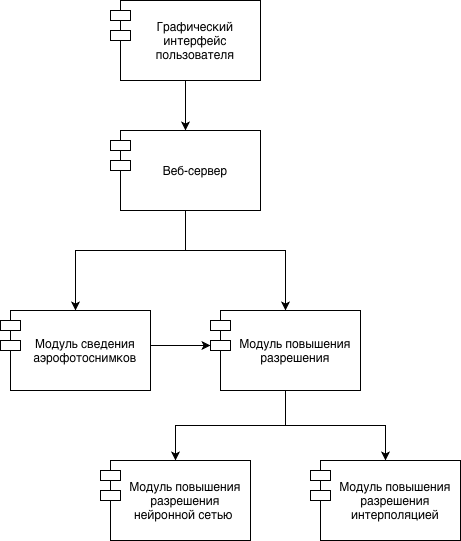
\includegraphics[width=0.7\linewidth]{images/technological/postruct.png}
    \caption{Структура ПО}
    \label{fig:tech:postruct}
\end{figure}

\section{Реализация алгоритма сведения изображений}

Реализация алгоритма сведения изображений с разными разрешениями к максимальному представлена в листингах~\ref{reduce}~---~\ref{_scale_images}. 

\mylisting[./static/lsts/reduce.py]{Функция сведения изображений}{}{label=reduce}

\mylisting[./static/lsts/scale.py]{Функция масштабирования изображений до нужного разрешения}{}{label=_scale_images}

% \section{Реализация алгоритма выбора коэффициента масштабирования нейронной сети}

% Реализация алгоритма сведения изображений с разными разрешениями к максимальному представлена в листинге~\ref{select}. 

% \mylisting[./static/lsts/select.py]{Функция выбора коэффициента масштабирования нейронной сети}{}{label=select}


\section{Тестирование программного обеспечения}

Графический интерфейс программного обеспечения представлен на рисунках~\ref{fig:tech:red_int}~---~\ref{fig:tech:scale_int}. Графический интерфейс позволяет:

\begin{itemize}[label=---]
    \item добавлять, удалять, очищать и просматривать выбранные для сведения изображения;
    \item просматривать одно изображение из сводимых;
    \item сводить изображения;
    \item просмотреть результат сведения изображений;
    \item скачать архив сведенных изображений;
    \item загрузить и просмотреть масштабируемое изображение;
    \item выбирать коэффициент масштабирования и метод масштабирования. Доступны следующие методы: метод ближайшего соседа, билинейная интерполяция, бикубическая интерполяция, интерполяция Ланцоша, разработанный метод;
    \item масштабировать выбранное изображение и сравнивать методы на основе выбранного изображения;
    \item просмотреть масштабированное изображение и скачать его. 
\end{itemize}

\begin{figure}[H]
    \centering
    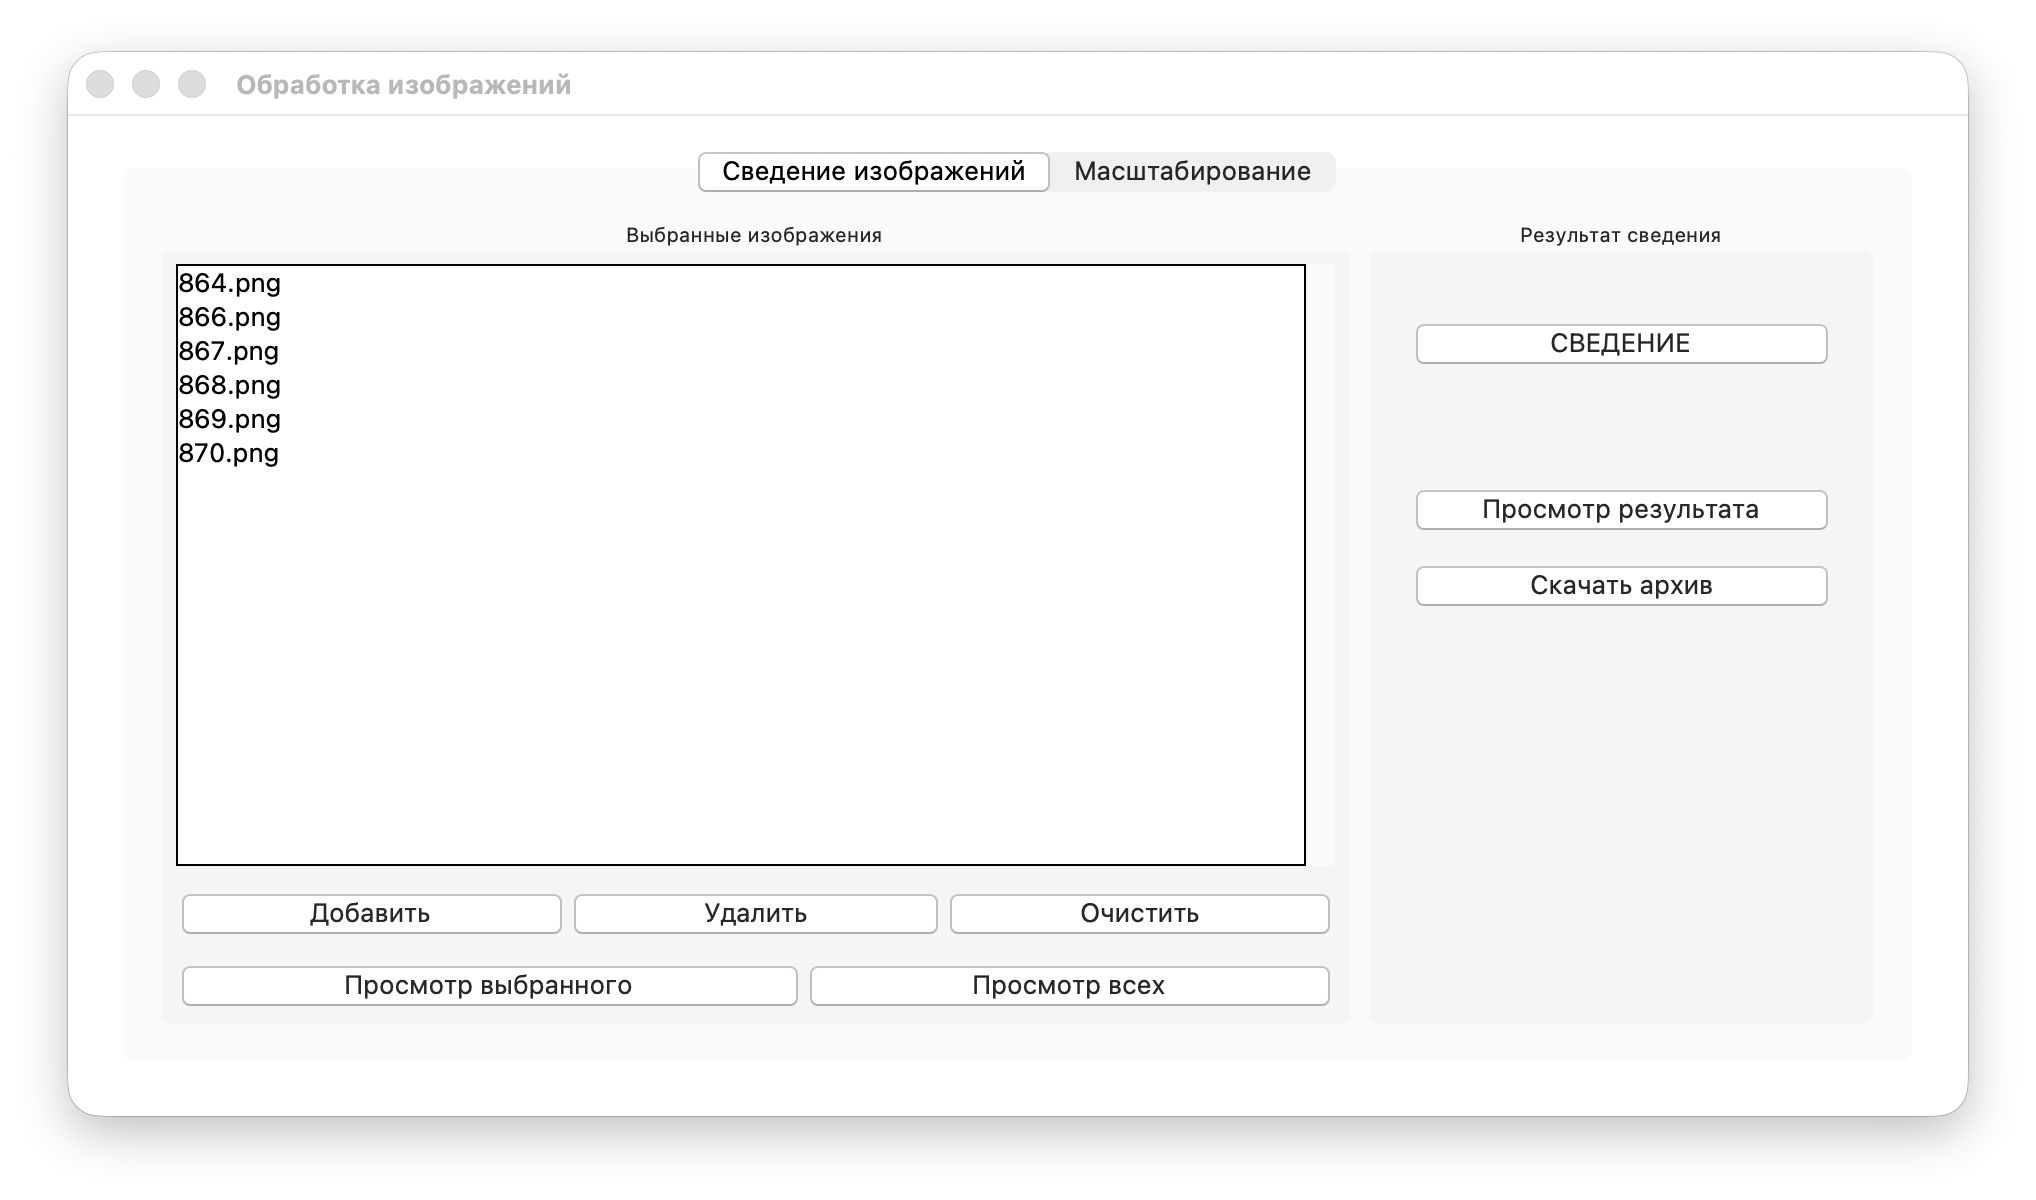
\includegraphics[width=0.8\linewidth]{images/technological/red_int.png}
    \caption{Вкладка сведения изображений}
    \label{fig:tech:red_int}
\end{figure}

\begin{figure}[H]
    \centering
    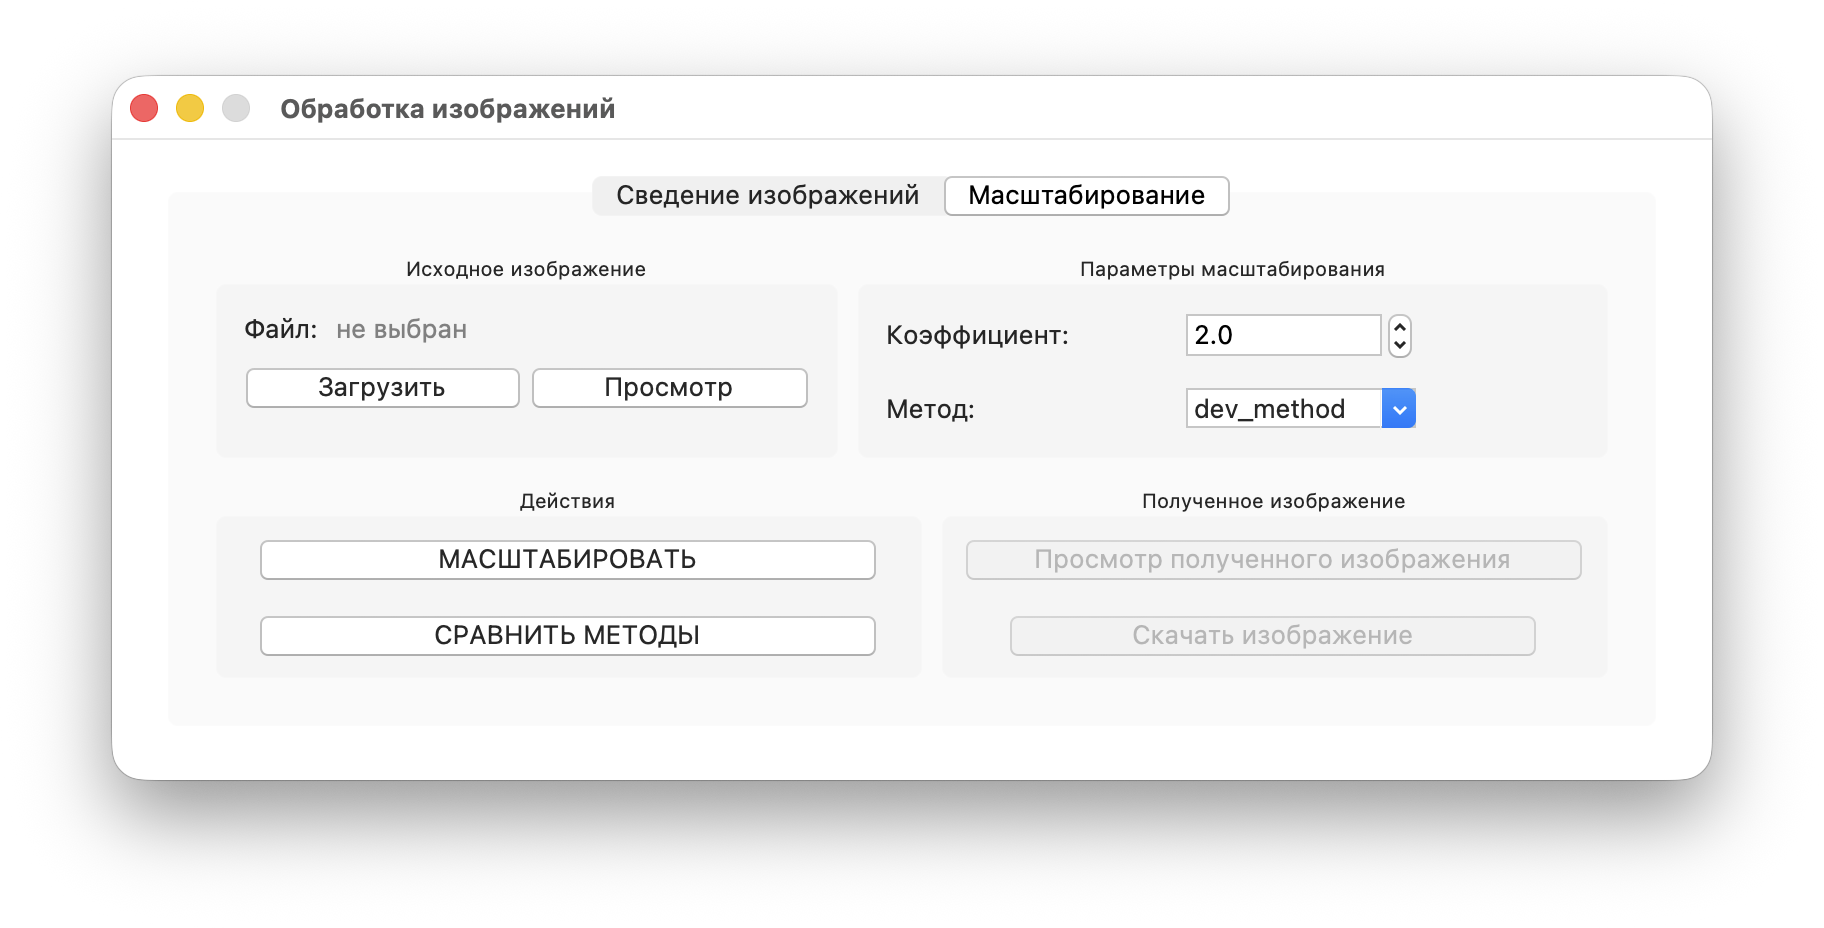
\includegraphics[width=0.8\linewidth]{images/technological/scale_int.png}
    \caption{Вкладка масштабирования изображения}
    \label{fig:tech:scale_int}
\end{figure}

Примеры работы сведения аэрофотоснимков представлены на рисунках~\ref{fig:tech:test3_in}~---~\ref{fig:tech:test6_out}. 

\begin{figure}[H]
    \centering
    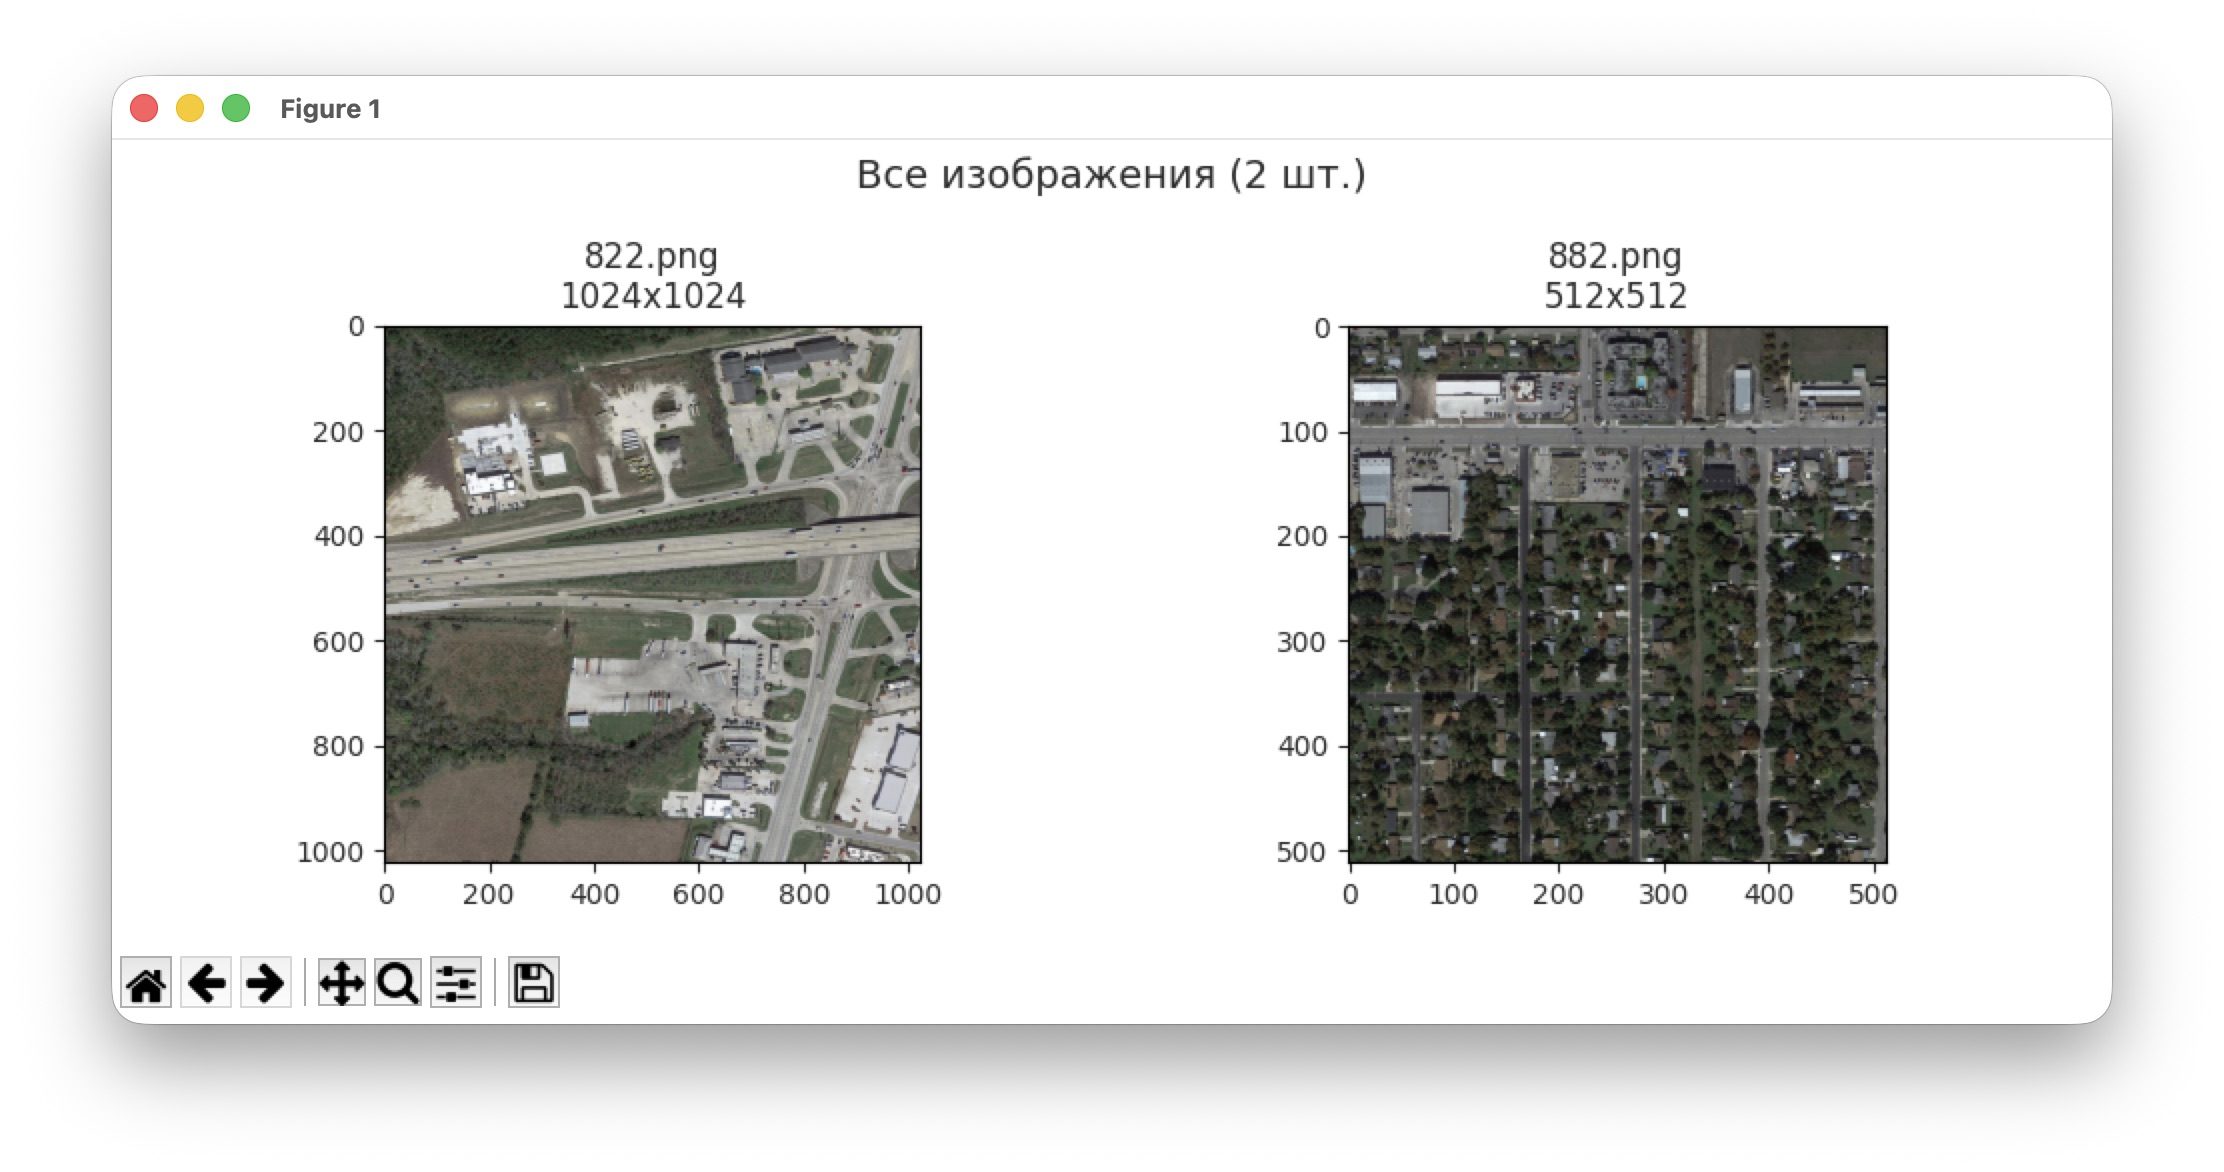
\includegraphics[width=0.9\linewidth]{images/technological/test3_in.jpeg}
    \caption{Два сводимых изображения}
    \label{fig:tech:test3_in}
\end{figure}

\begin{figure}[H]
    \centering
    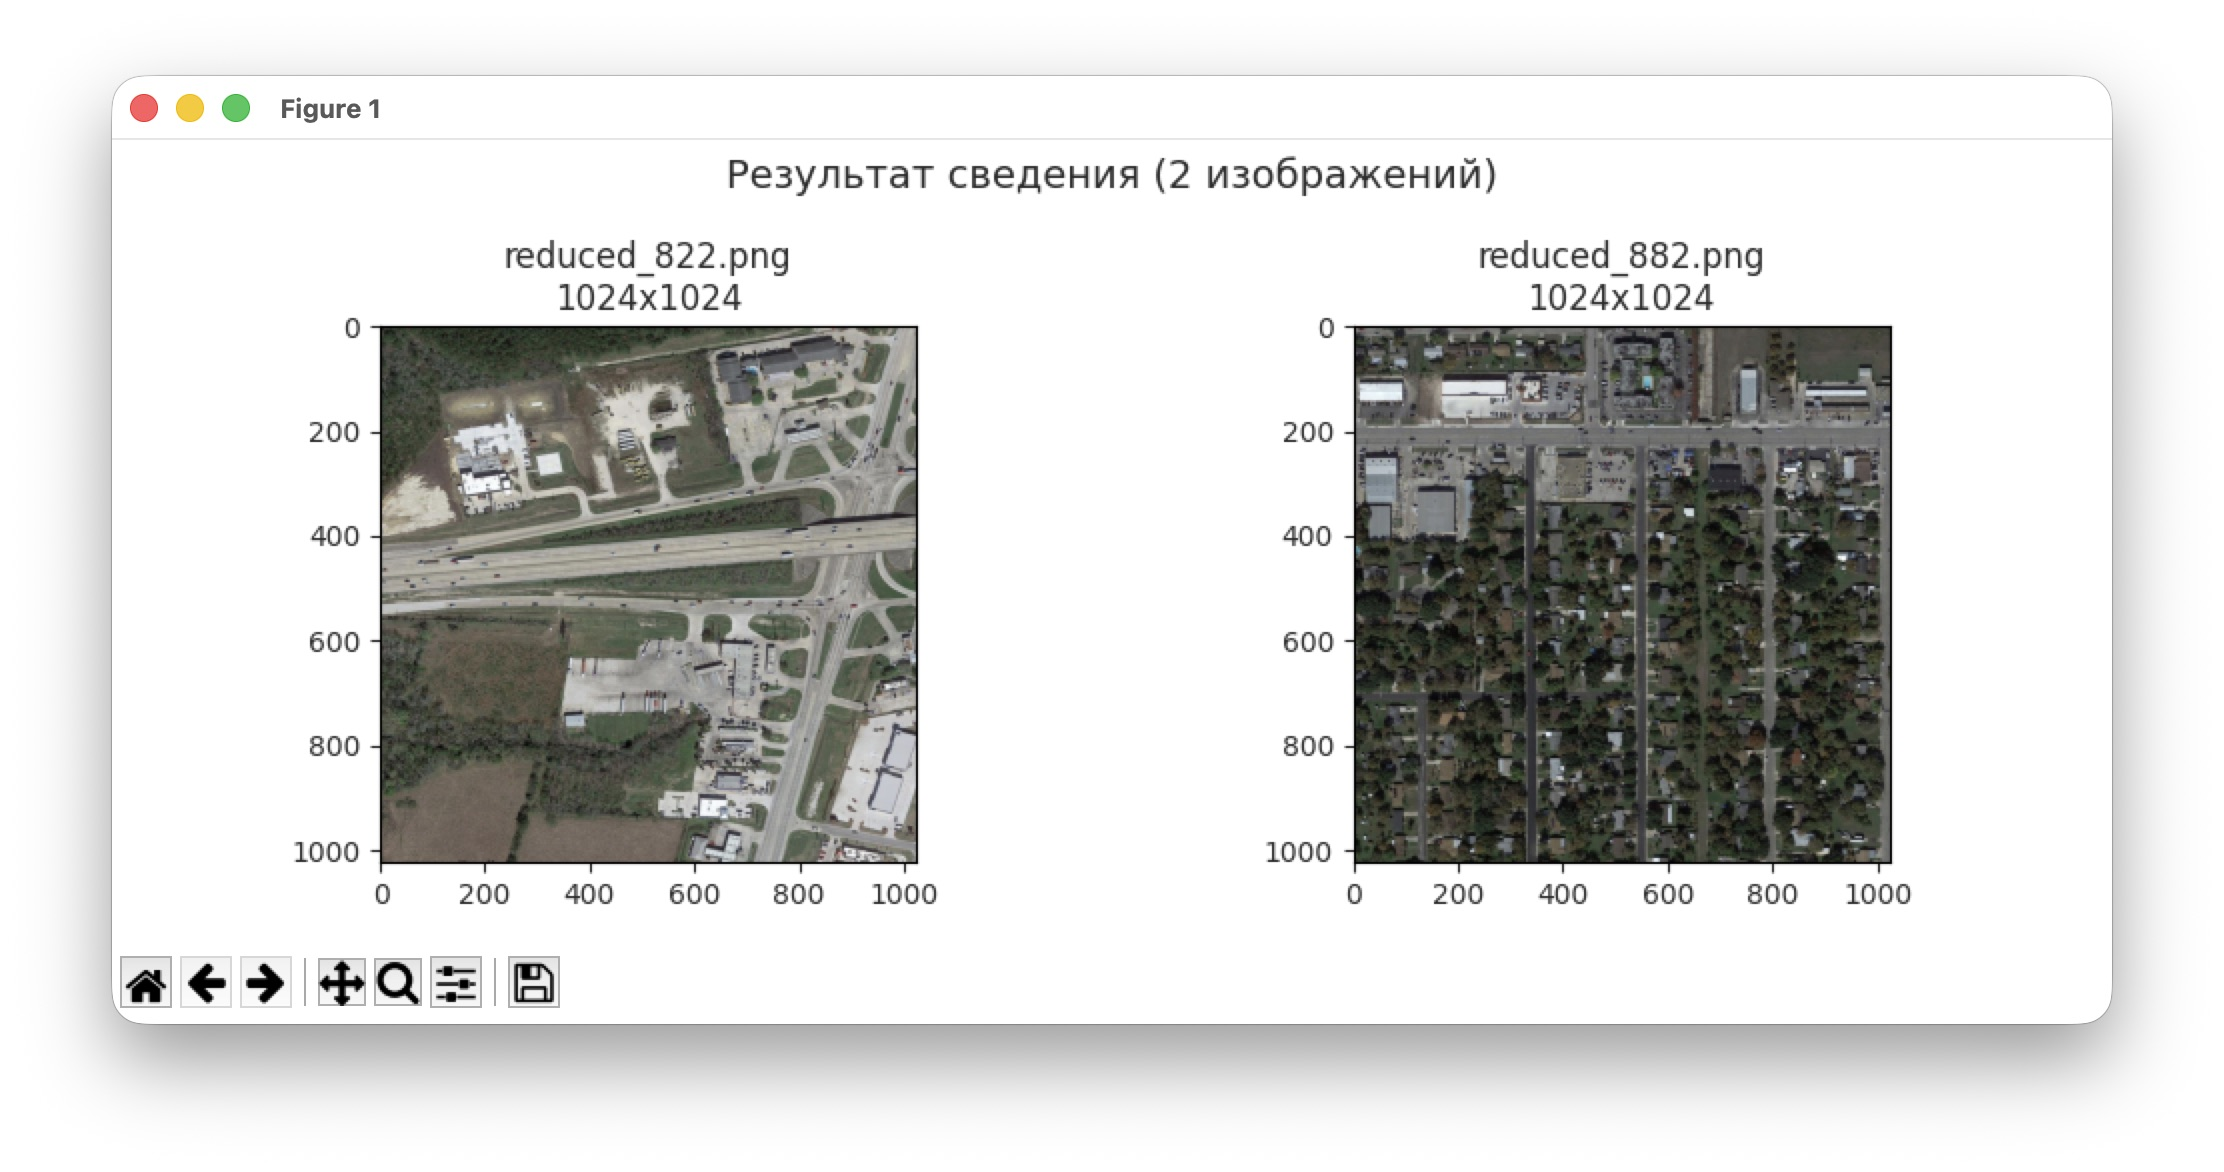
\includegraphics[width=0.9\linewidth]{images/technological/test3_out.jpeg}
    \caption{Результат сведения двух изображений}
    \label{fig:tech:test3_out}
\end{figure}

\begin{figure}[H]
    \centering
    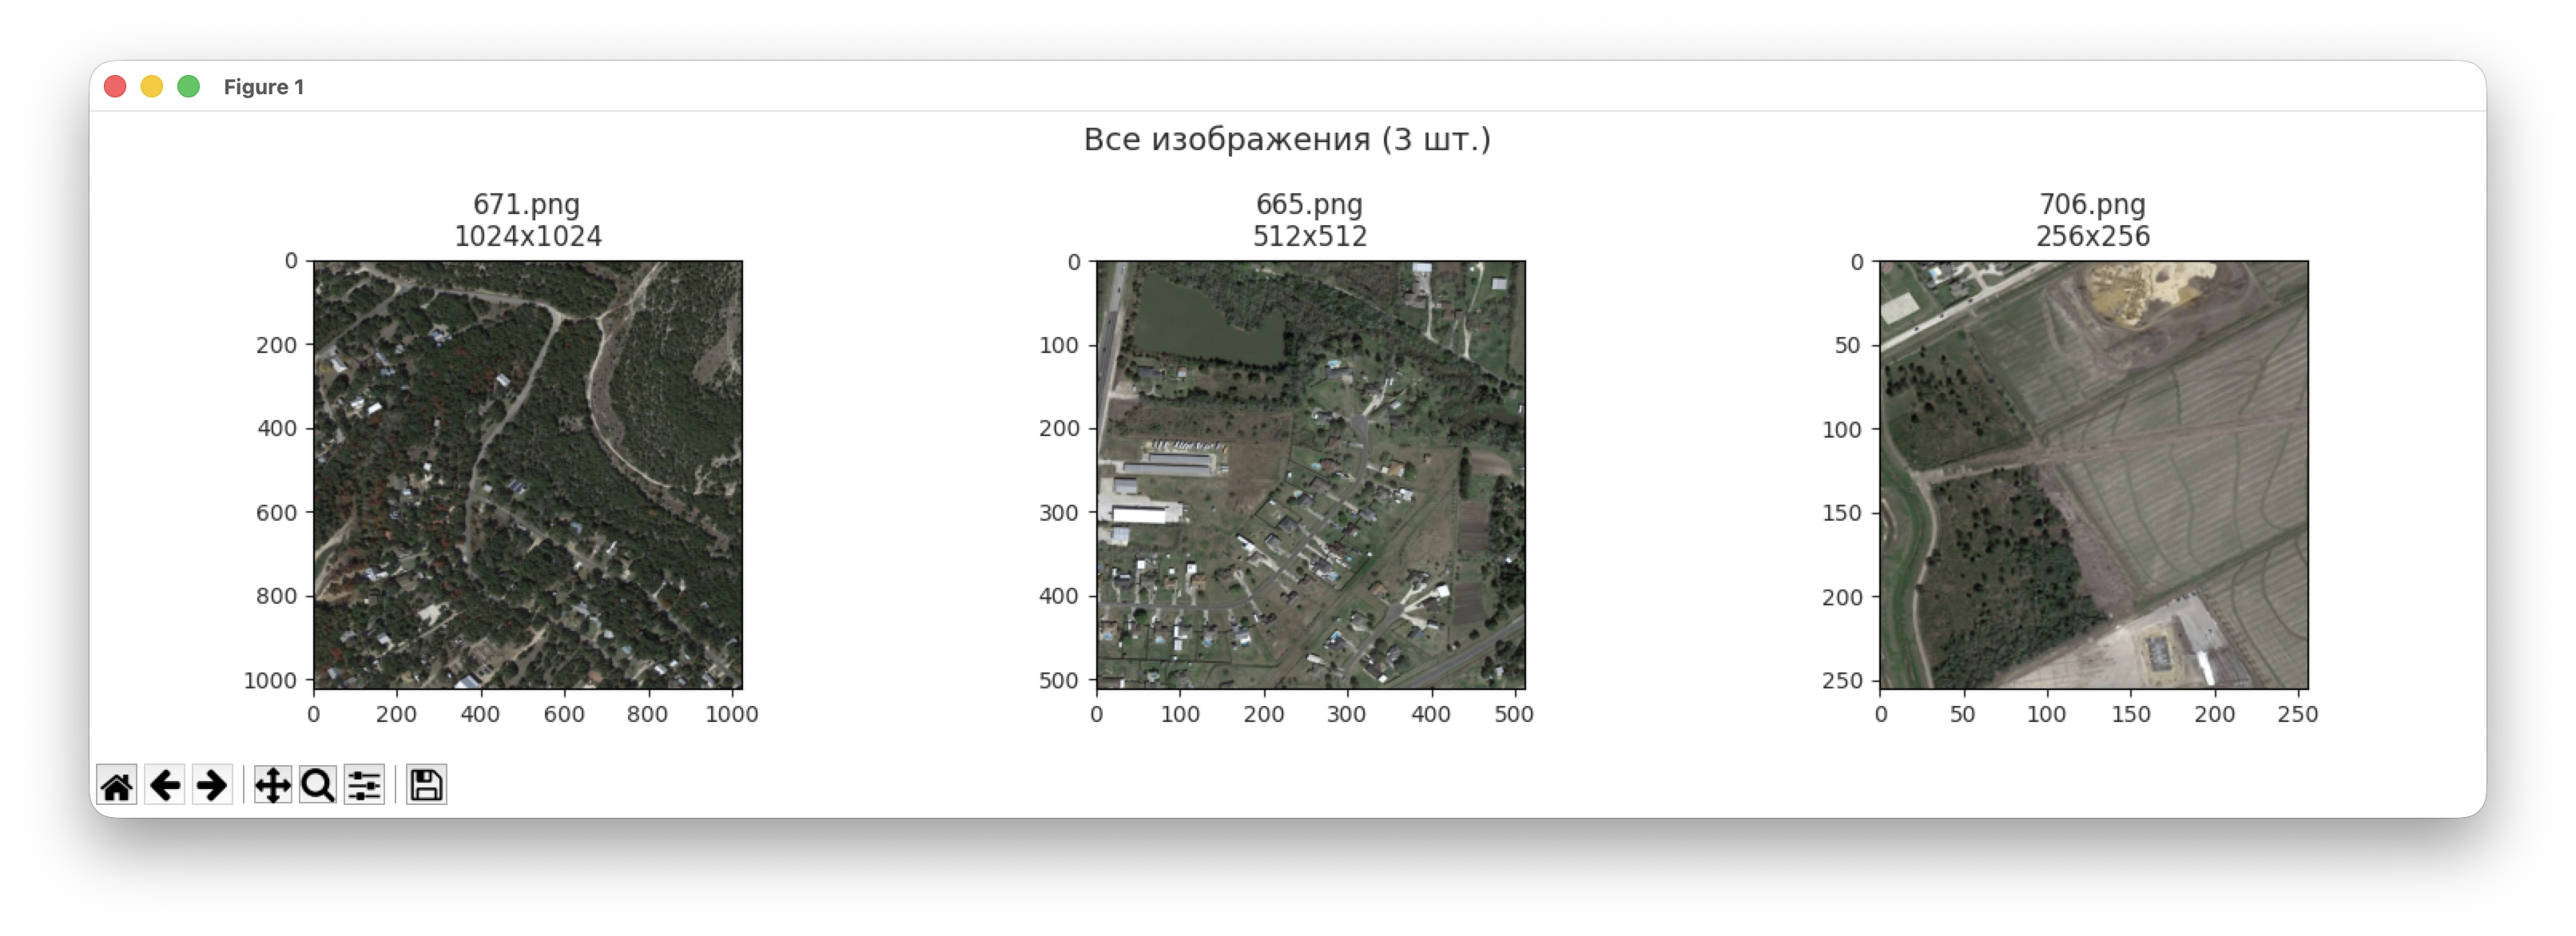
\includegraphics[width=0.9\linewidth]{images/technological/test2_in.jpeg}
    \caption{Три сводимых изображения с разными разрешениями}
    \label{fig:tech:test2_in}
\end{figure}

\begin{figure}[H]
    \centering
    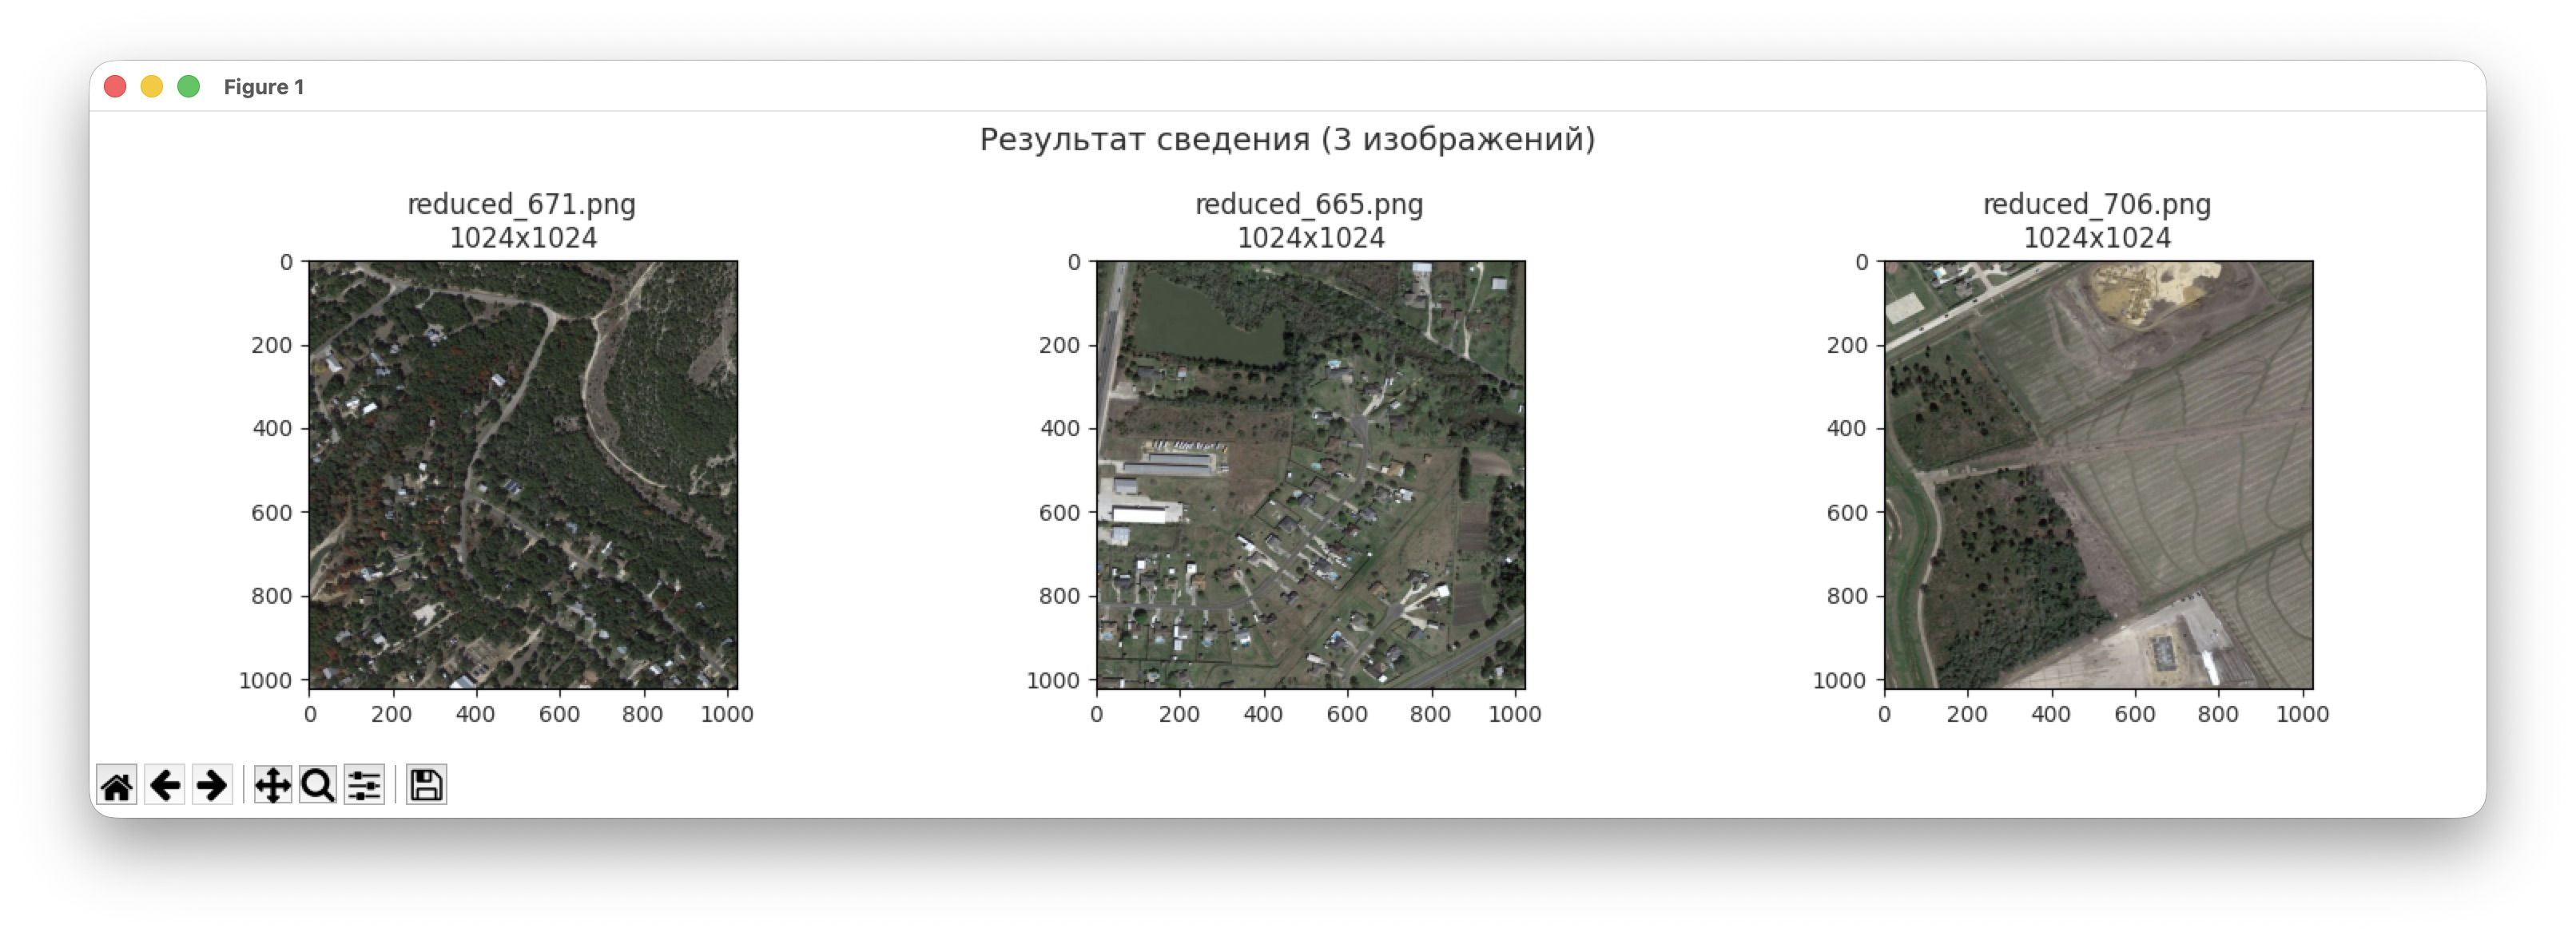
\includegraphics[width=0.9\linewidth]{images/technological/test2_out.jpeg}
    \caption{Результат сведения трех изображений с разными разрешениями}
    \label{fig:tech:test2_out}
\end{figure}

\begin{figure}[H]
    \centering
    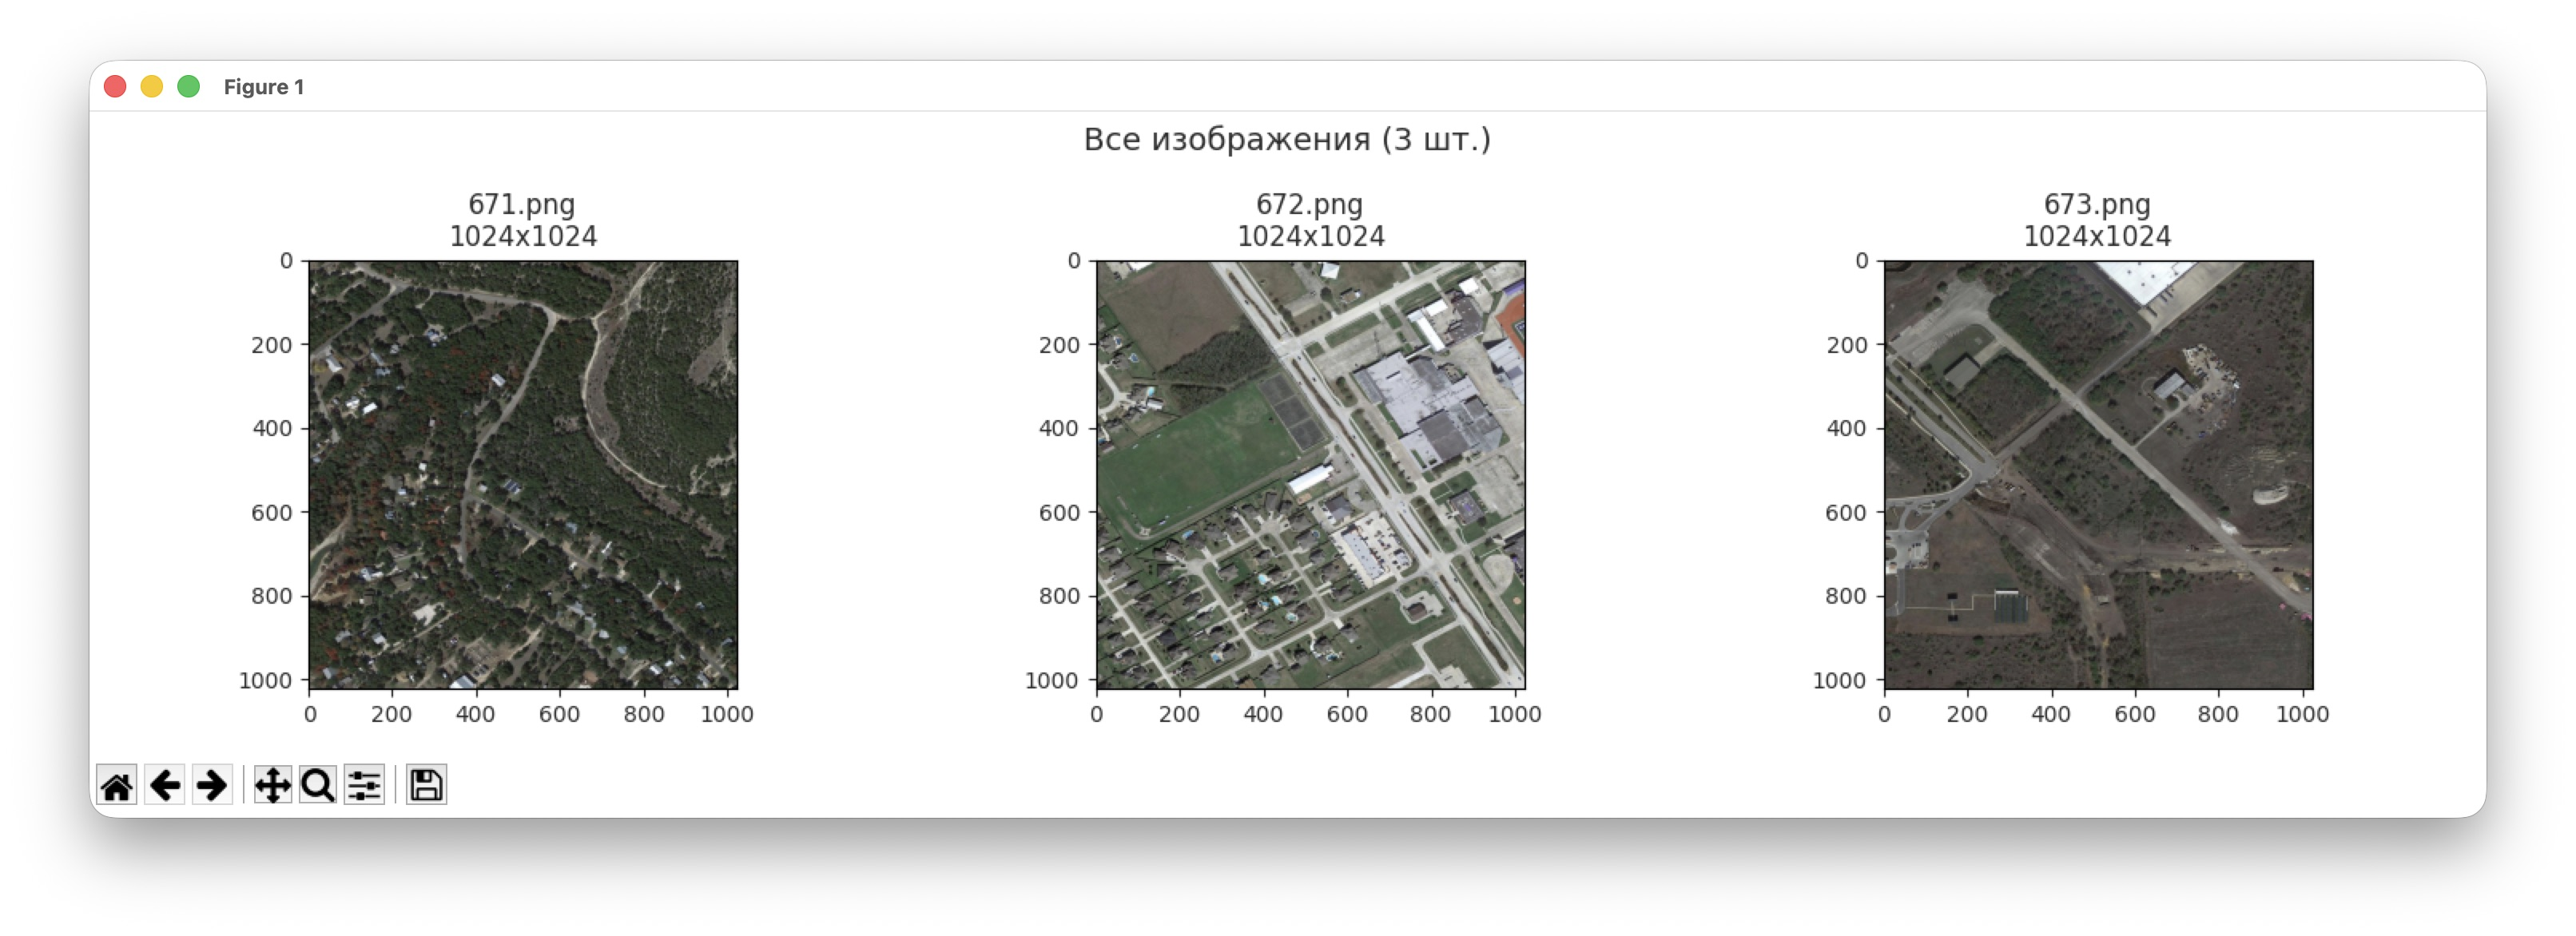
\includegraphics[width=0.9\linewidth]{images/technological/test1_in.jpeg}
    \caption{Три сводимых изображения с одинаковыми разрешениями}
    \label{fig:tech:test1_in}
\end{figure}

\begin{figure}[H]
    \centering
    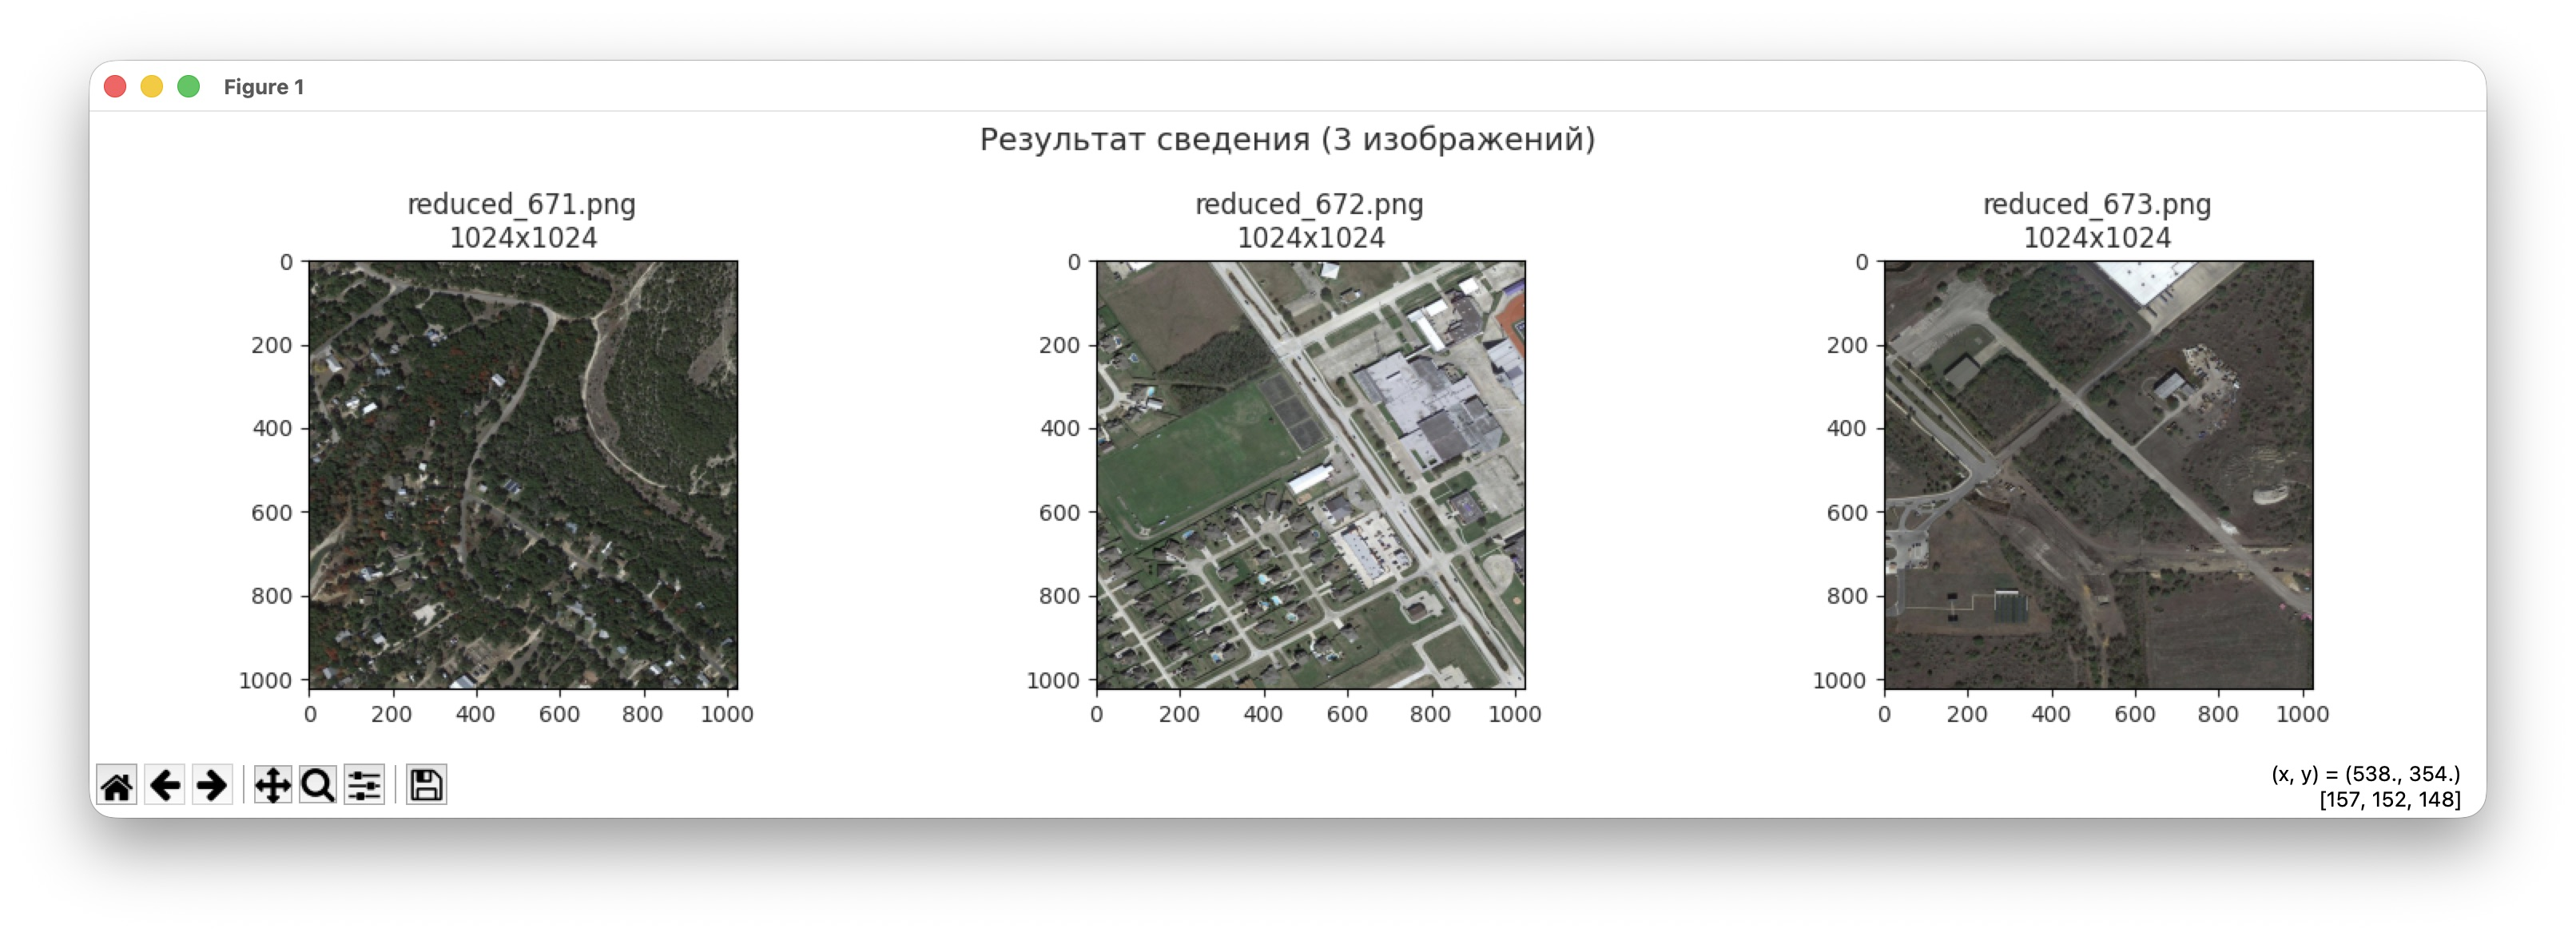
\includegraphics[width=0.9\linewidth]{images/technological/test1_out.jpeg}
    \caption{Результат сведения трех изображений с одинаковыми разрешениями}
    \label{fig:tech:test1_out}
\end{figure}

\begin{figure}[H]
    \centering
    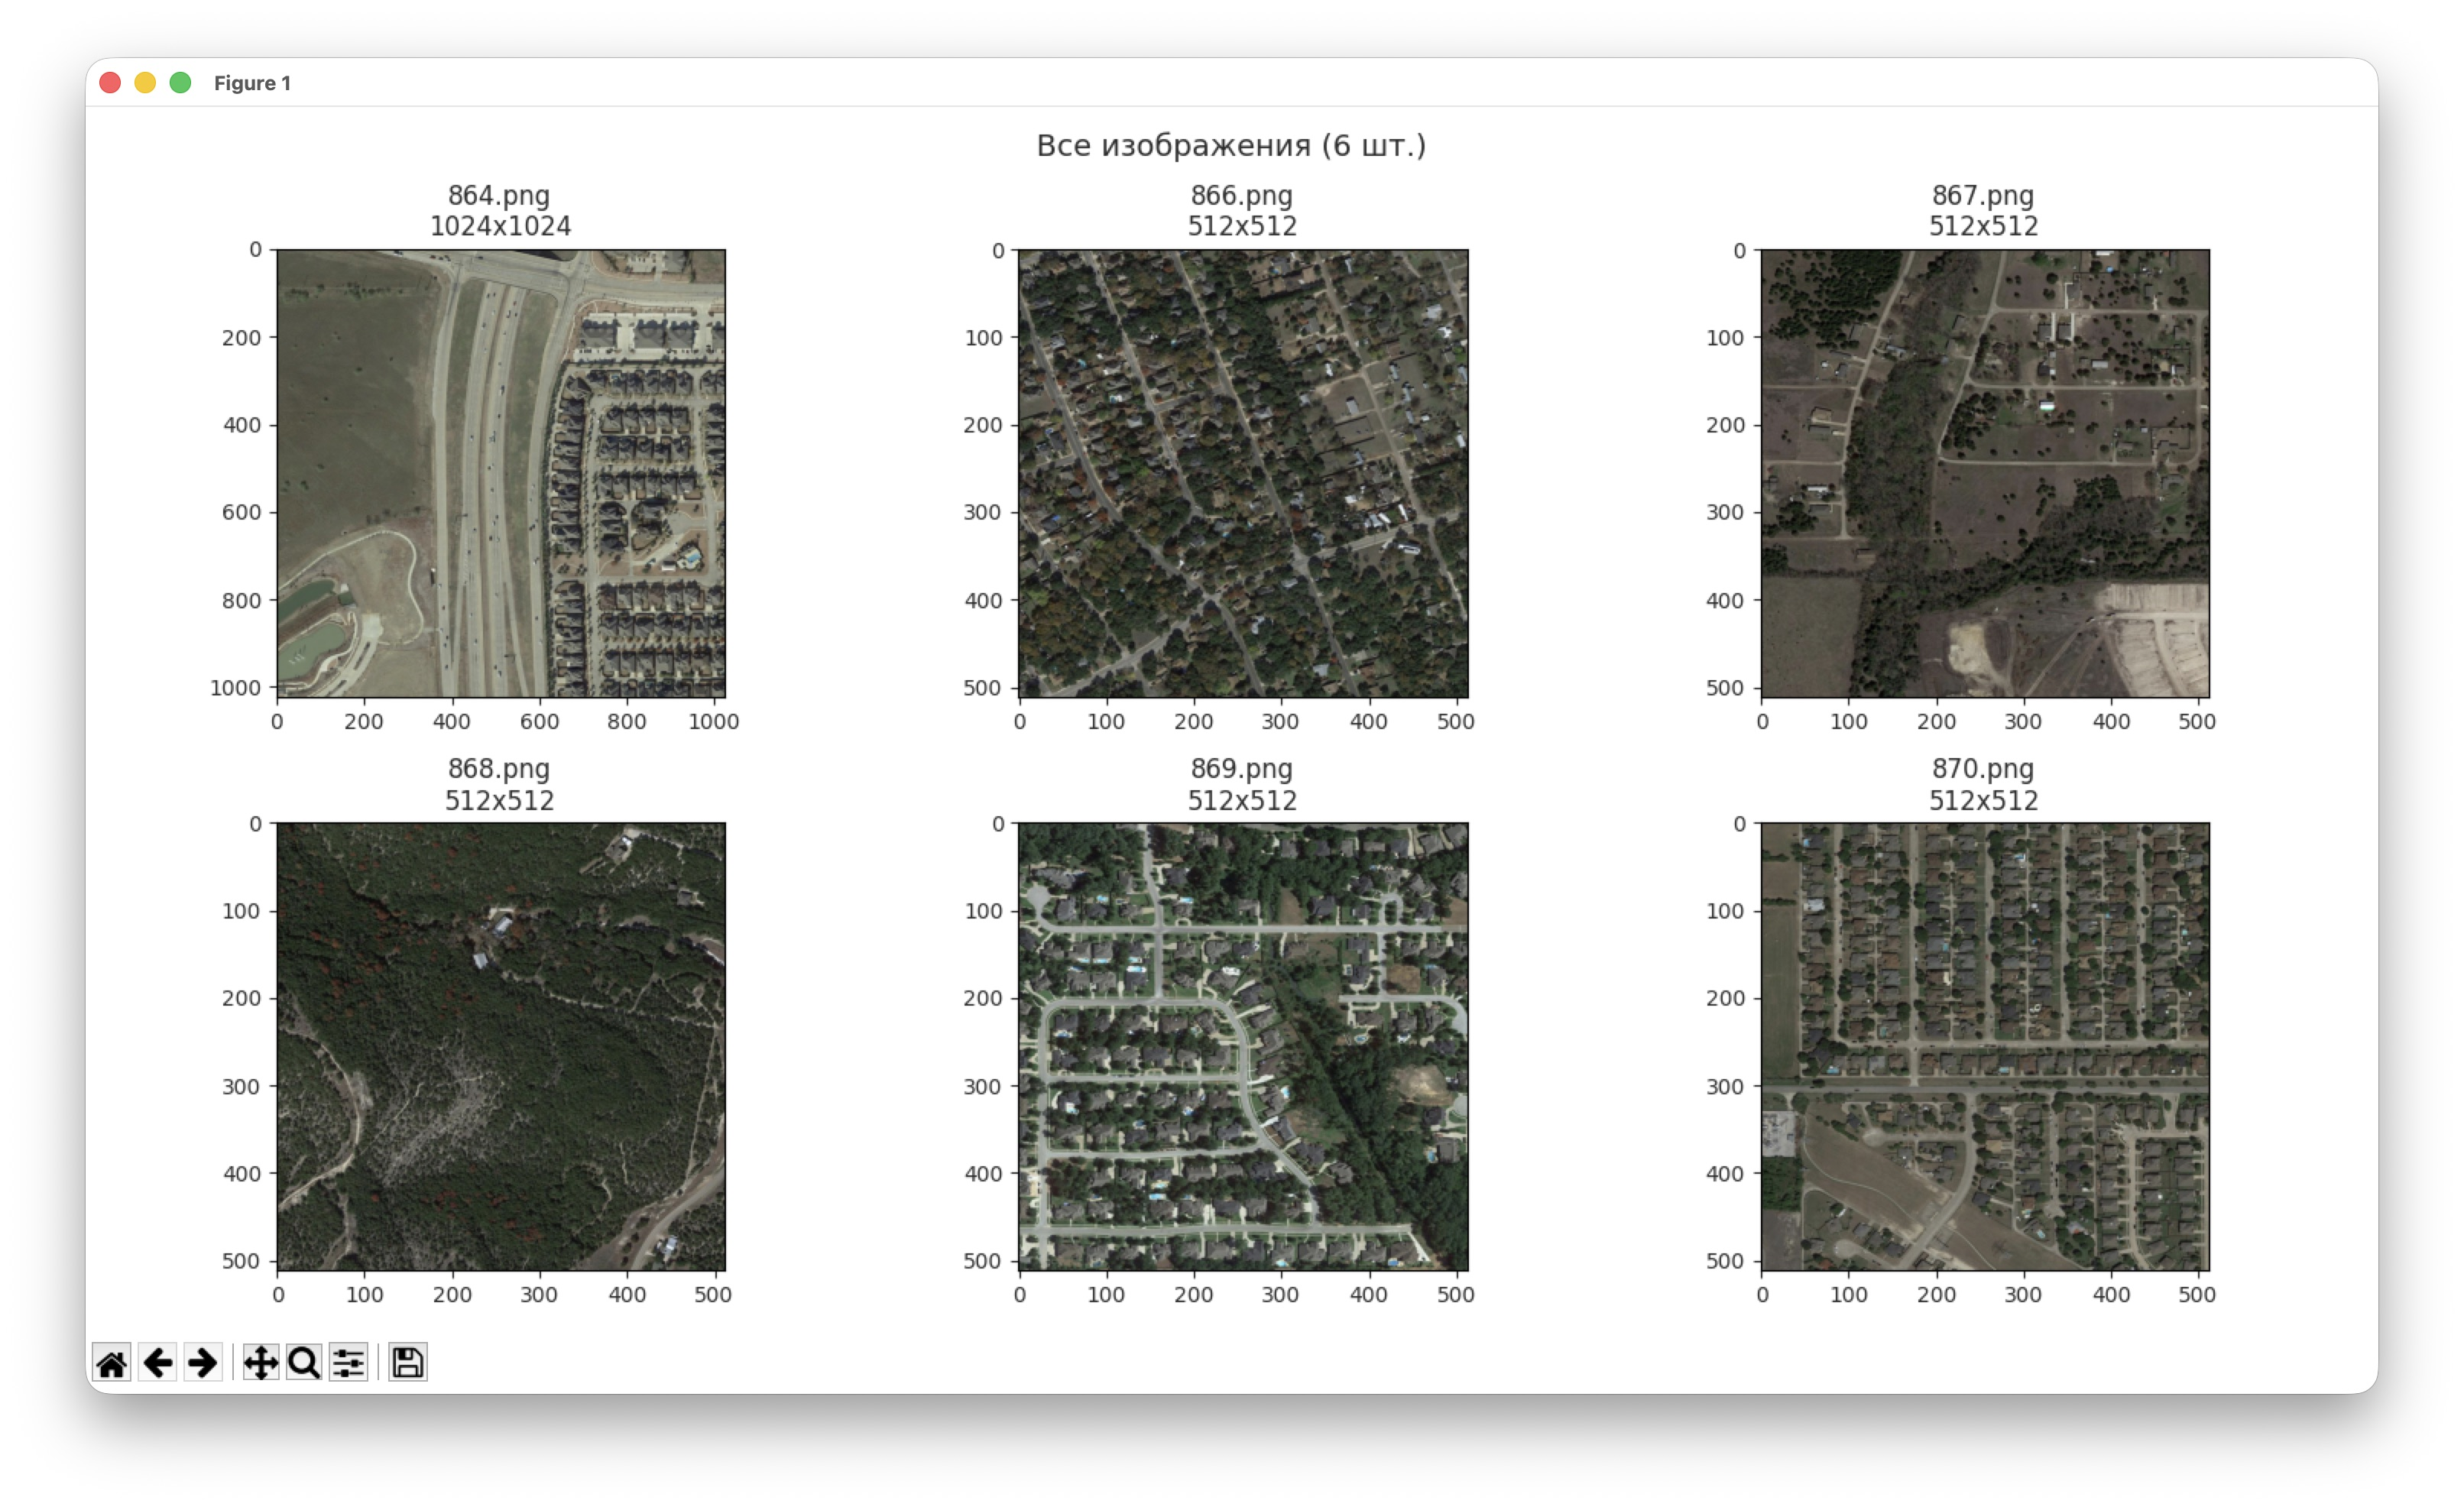
\includegraphics[width=0.9\linewidth]{images/technological/test4_in.jpeg}
    \caption{Шесть сводимых изображений}
    \label{fig:tech:test4_in}
\end{figure}

\begin{figure}[H]
    \centering
    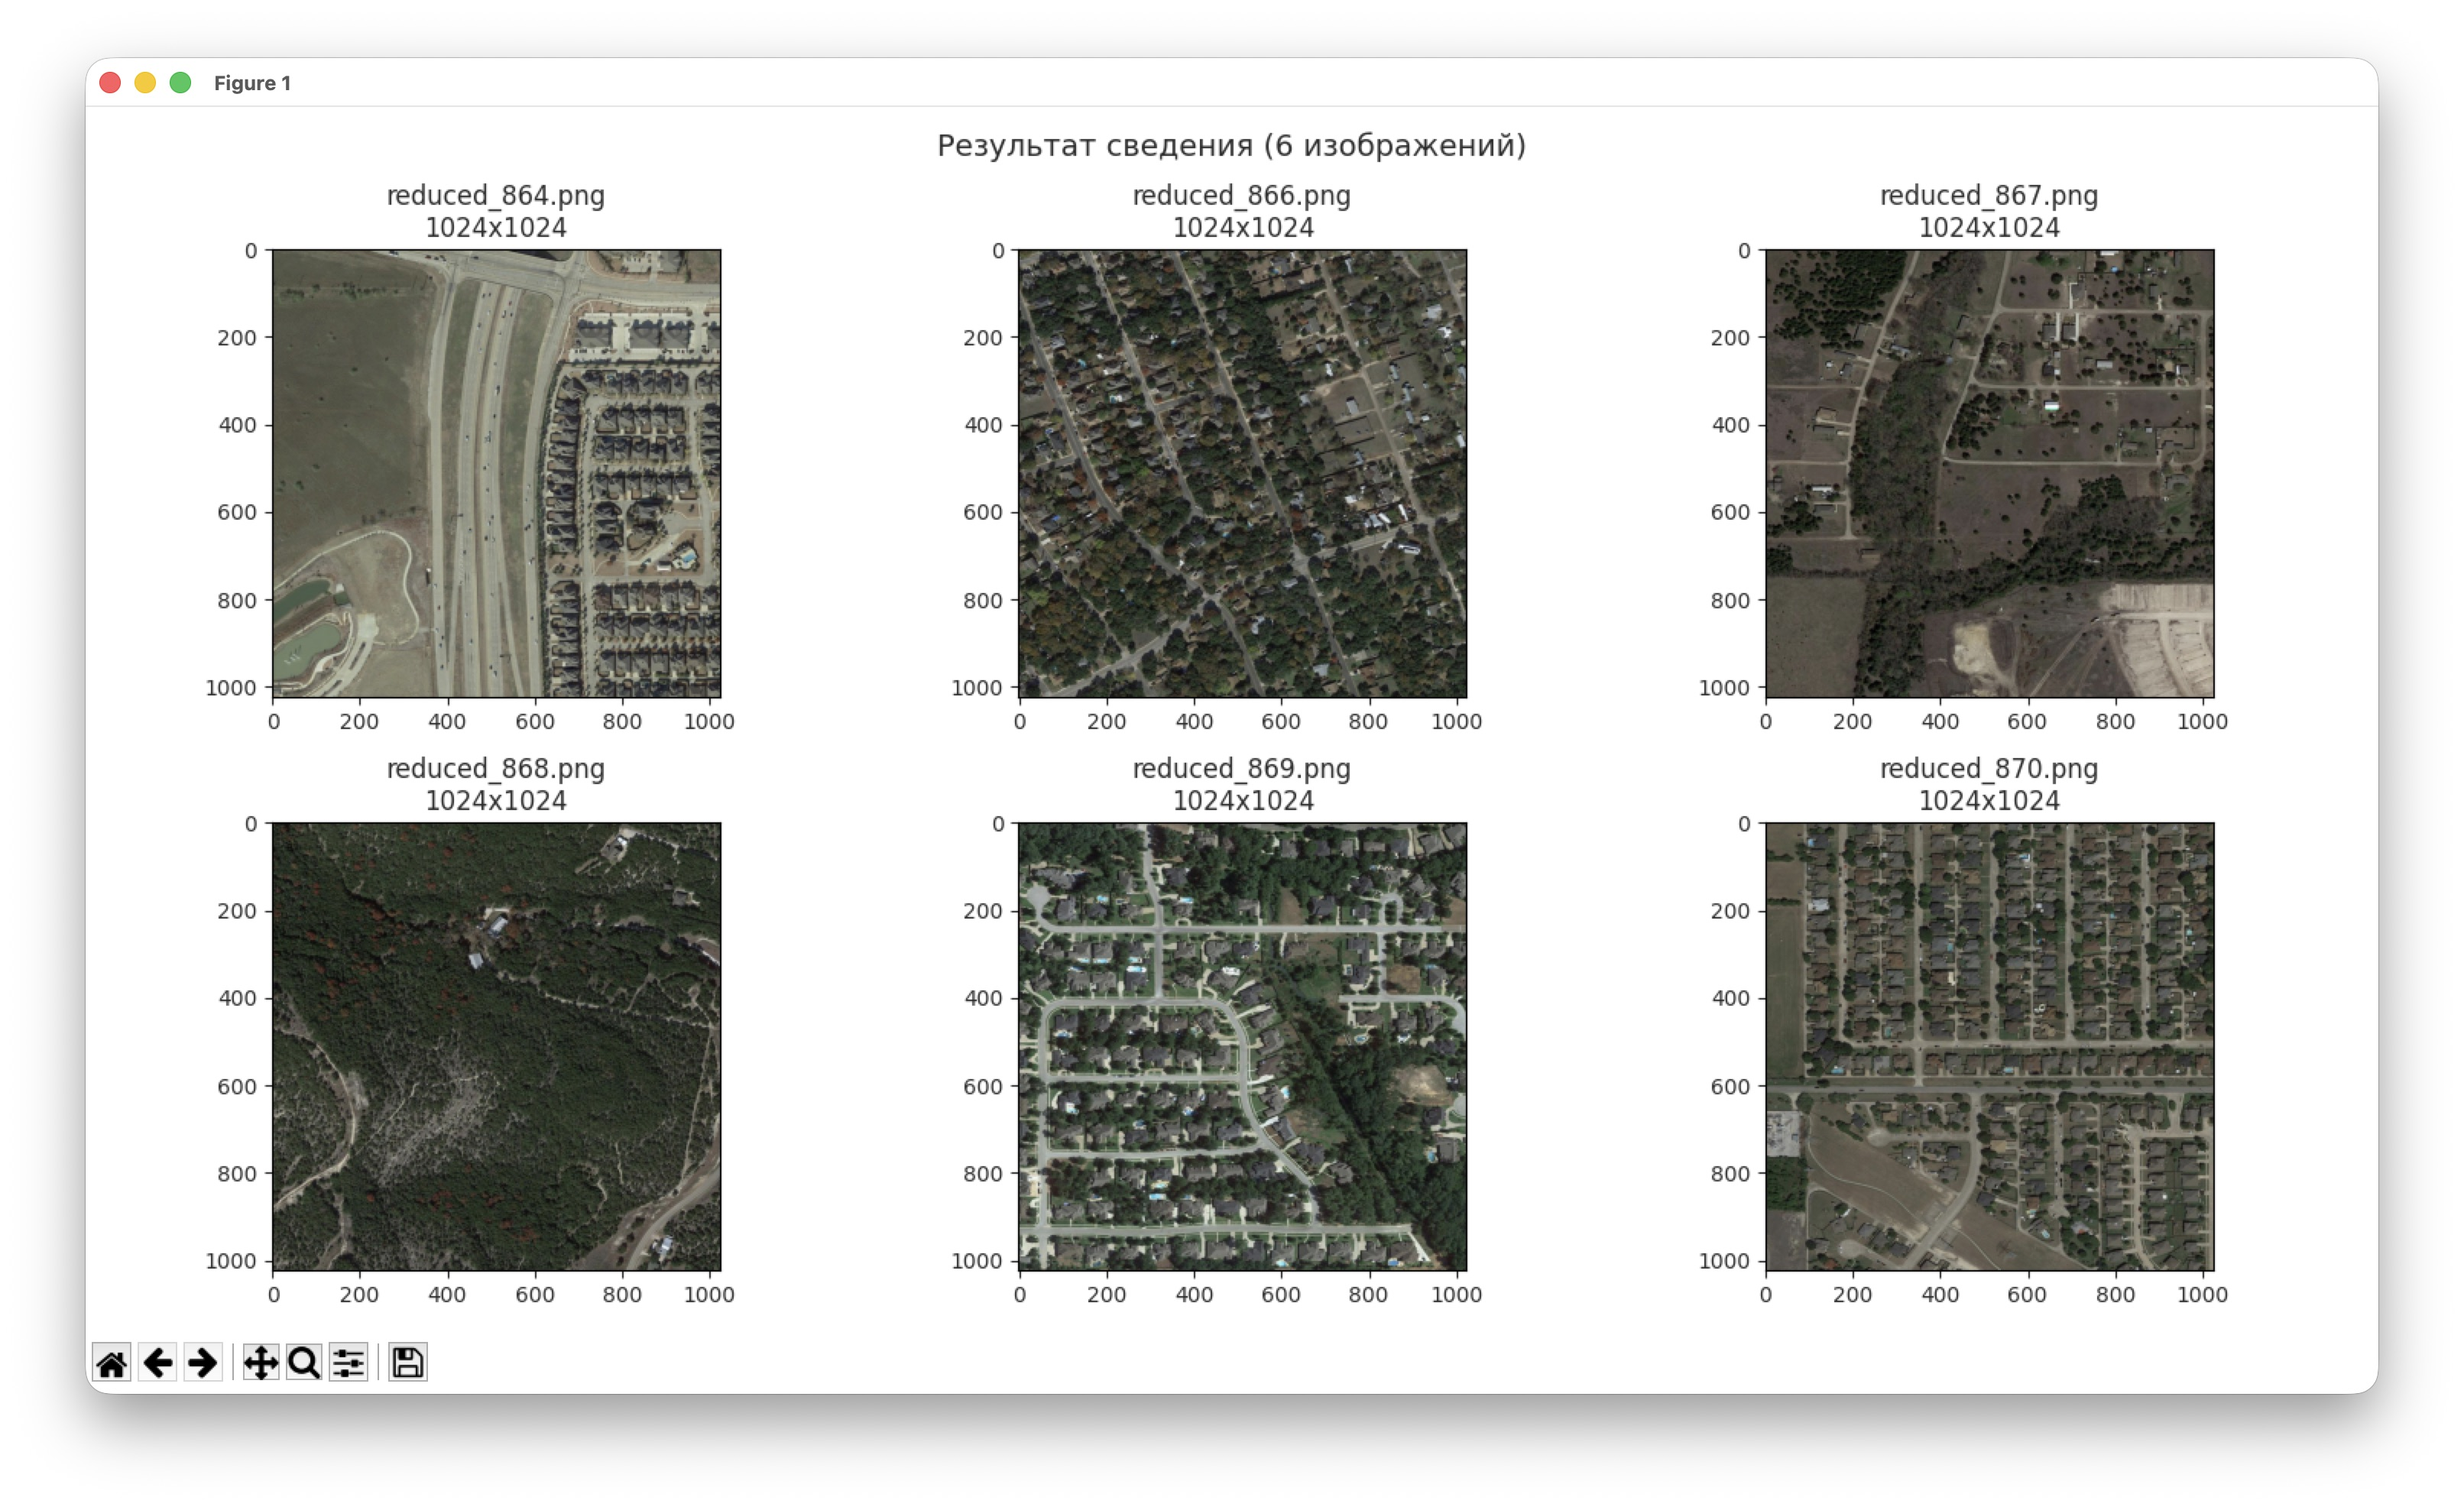
\includegraphics[width=0.9\linewidth]{images/technological/test4_out.jpeg}
    \caption{Результат сведения шести изображений}
    \label{fig:tech:test4_out}
\end{figure}

\begin{figure}[H]
    \centering
    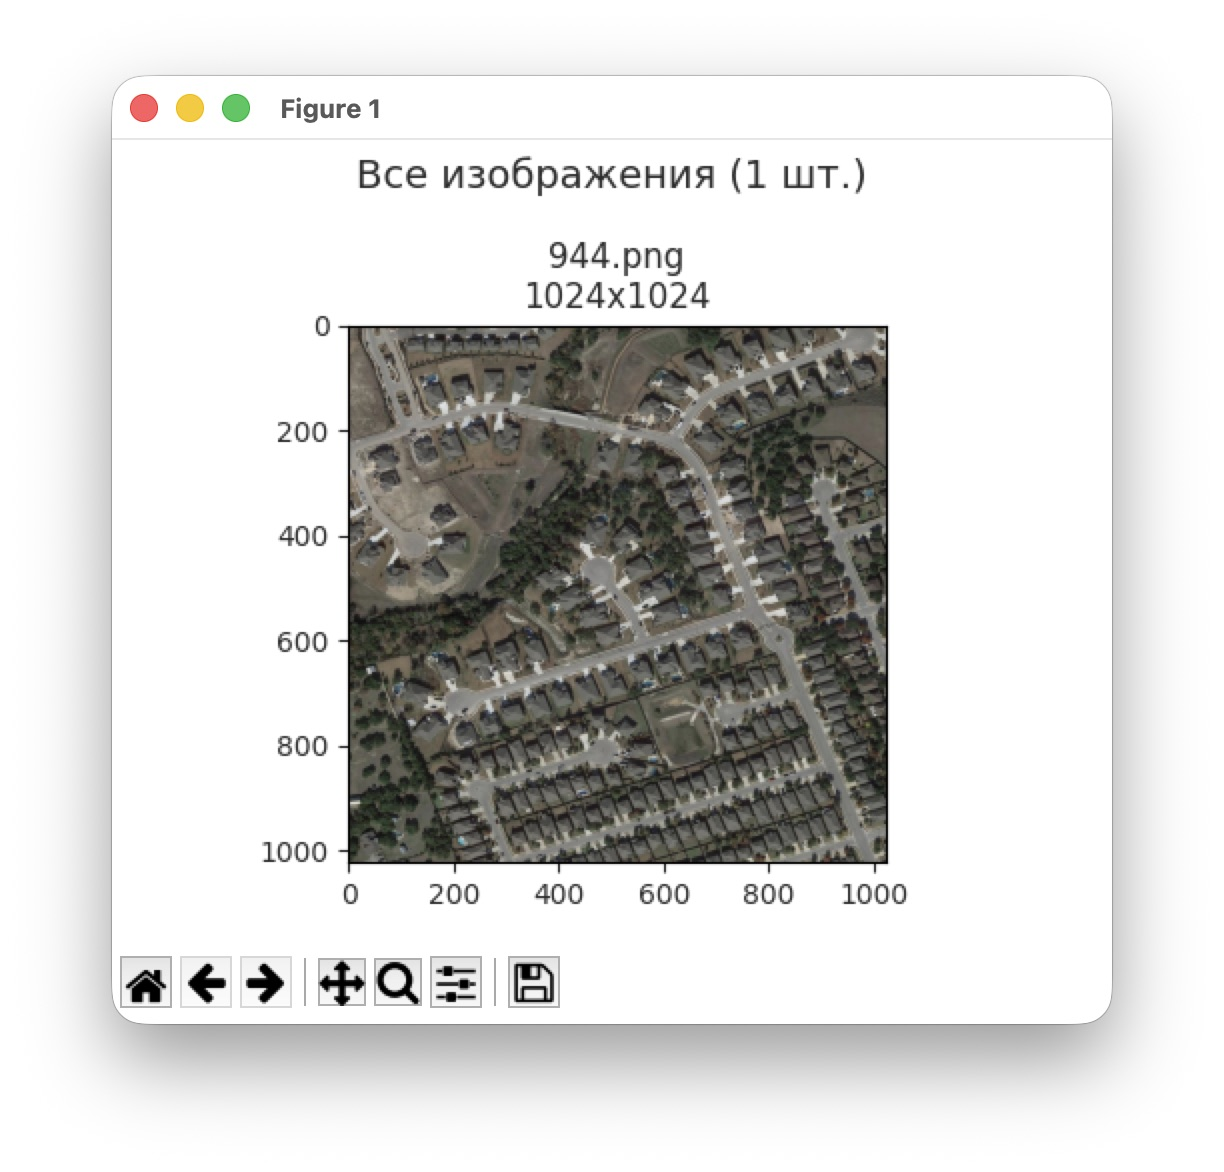
\includegraphics[width=0.6\linewidth]{images/technological/test5_in.jpeg}
    \caption{Сведение одного изображения}
    \label{fig:tech:test5_in}
\end{figure}

\begin{figure}[H]
    \centering
    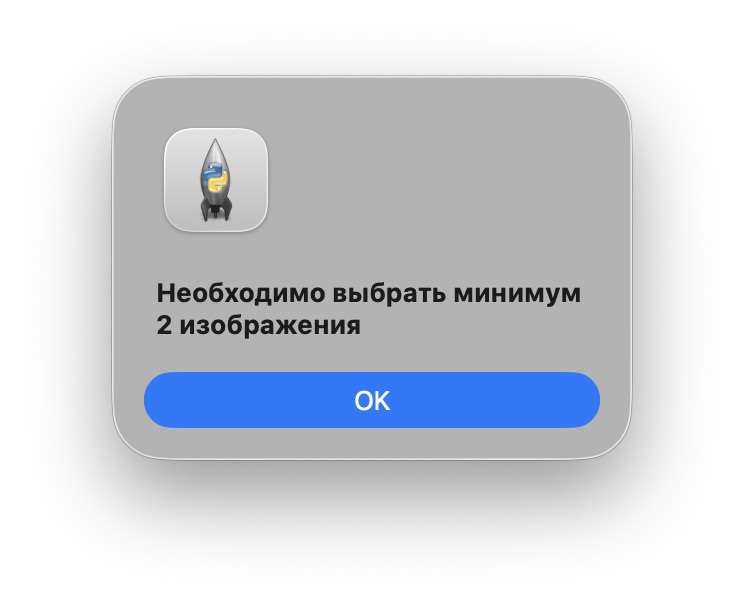
\includegraphics[width=0.6\linewidth]{images/technological/test5_out.jpeg}
    \caption{Ошибка сведения одного изображения}
    \label{fig:tech:test5_out}
\end{figure}

\begin{figure}[H]
    \centering
    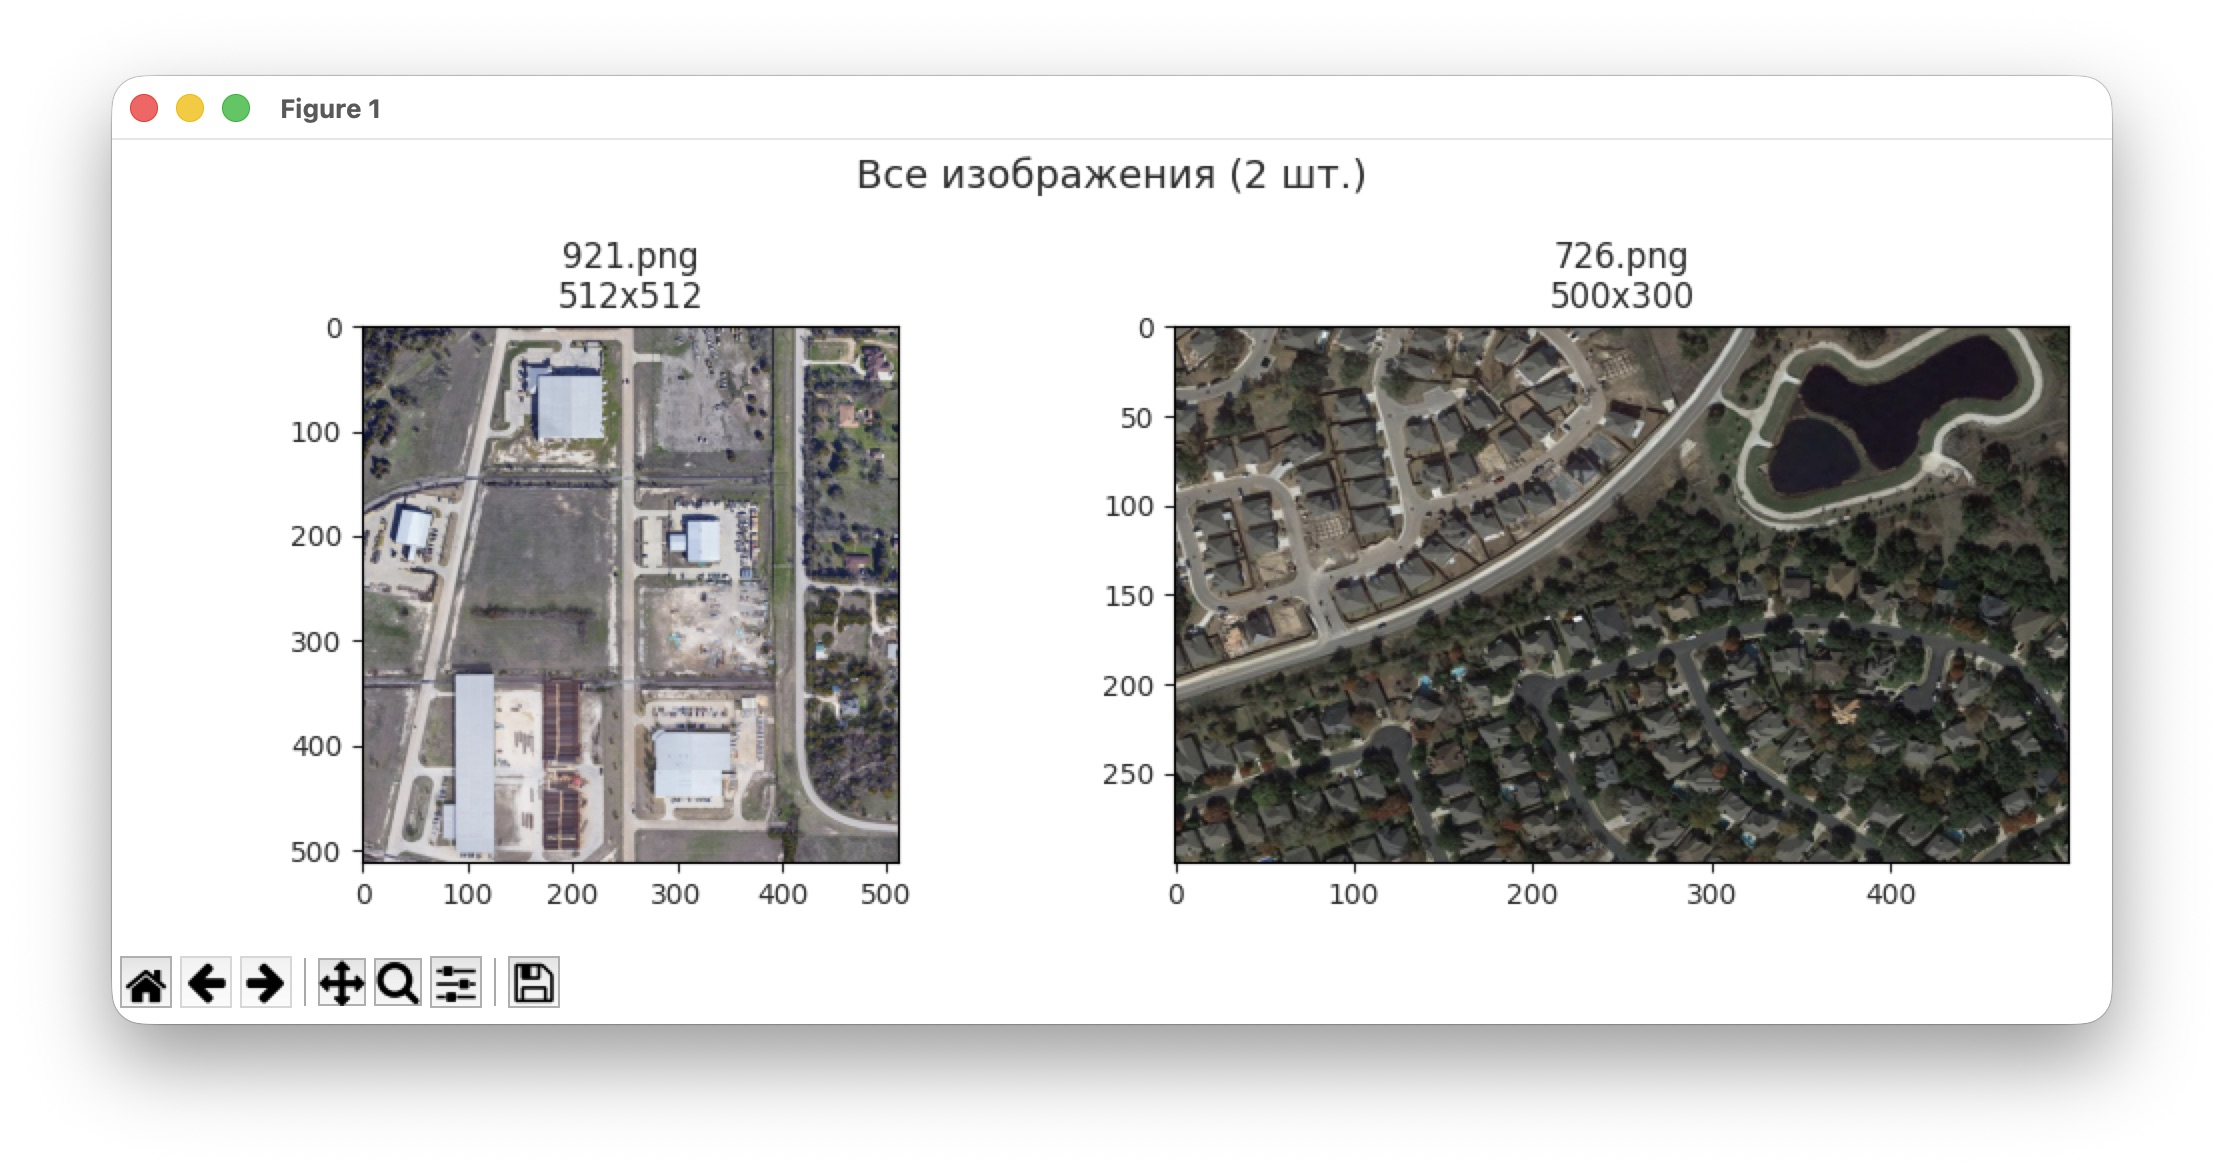
\includegraphics[width=0.9\linewidth]{images/technological/test6_in.jpeg}
    \caption{Сведение изображений с разными разрешениями}
    \label{fig:tech:test6_in}
\end{figure}

\begin{figure}[H]
    \centering
    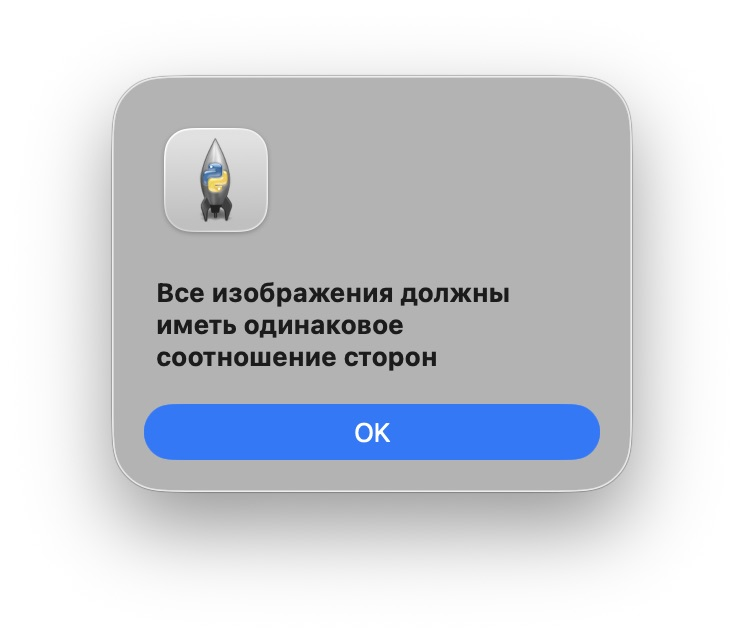
\includegraphics[width=0.6\linewidth]{images/technological/test6_out.jpeg}
    \caption{Ошибка сведения изображений с разными разрешениями}
    \label{fig:tech:test6_out}
\end{figure}

Исходя из примеров работы сведения аэрофотоснимков видно что метод корректно определяет максимальное разрешение, работает при разном количестве входных изображений и корректно обрабатывает ошибки.

На рисунках~\ref{fig:tech:test_s1_in}~---~\ref{fig:tech:test_s5_out} представлены примеры работы масштабирования аэрофотоснимков.

\begin{figure}[H]
    \centering
    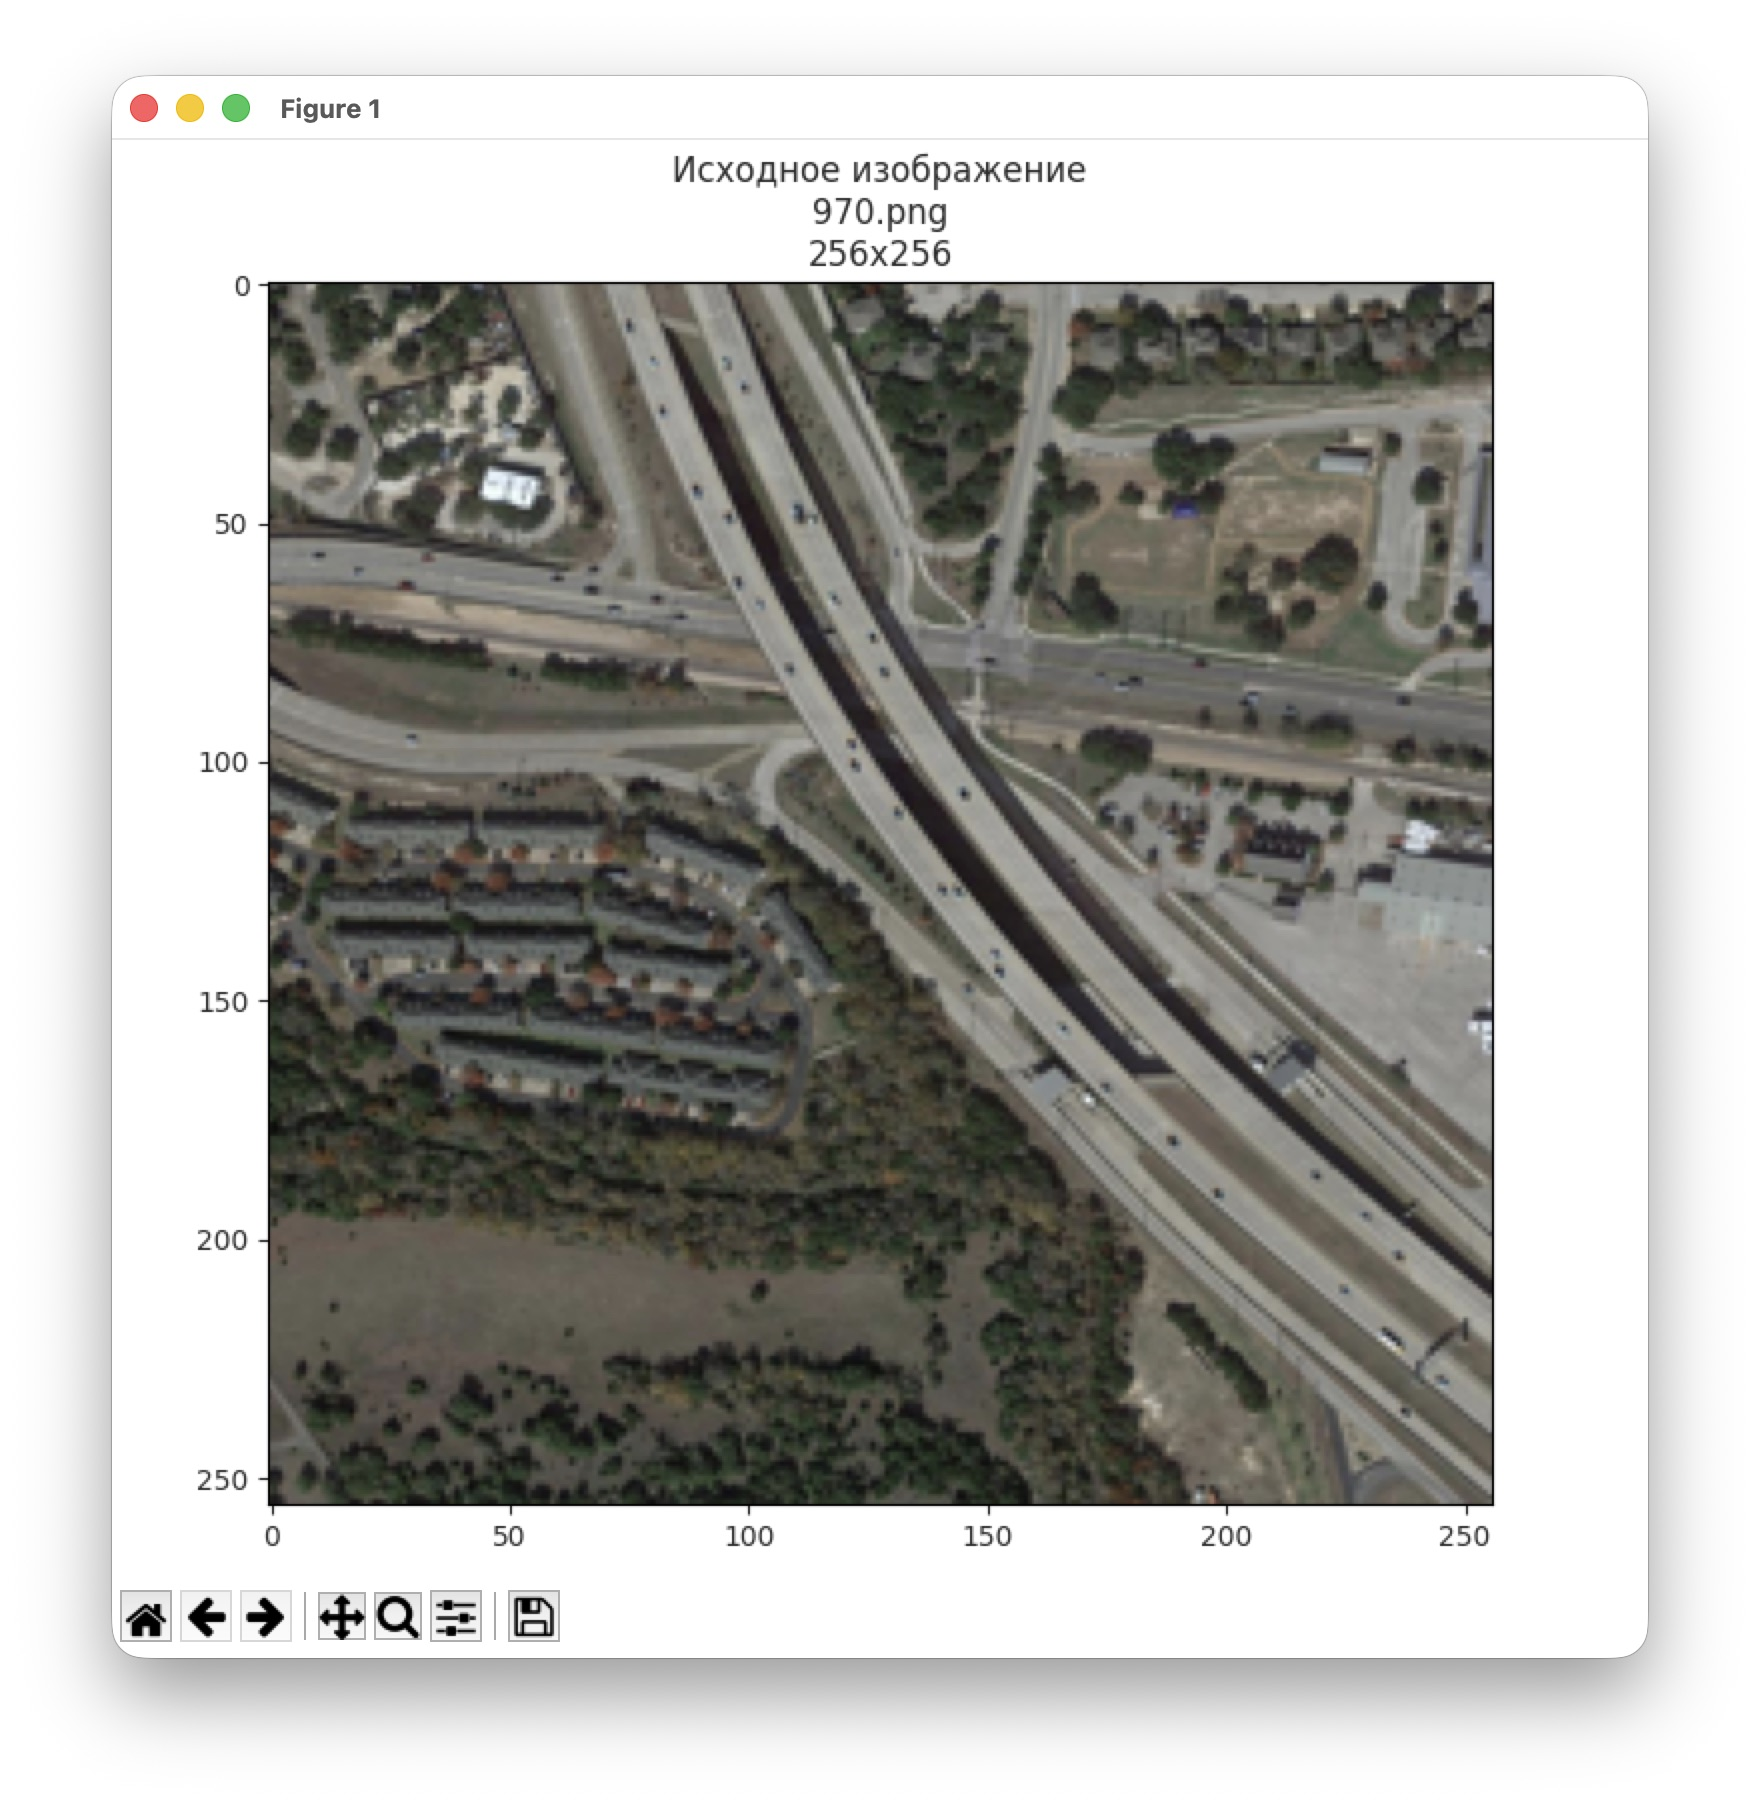
\includegraphics[width=0.6\linewidth]{images/technological/test_s1_in.jpeg}
    \caption{Входное изображение с разрешением $256 \times 256$}
    \label{fig:tech:test_s1_in}
\end{figure}

\begin{figure}[H]
    \centering
    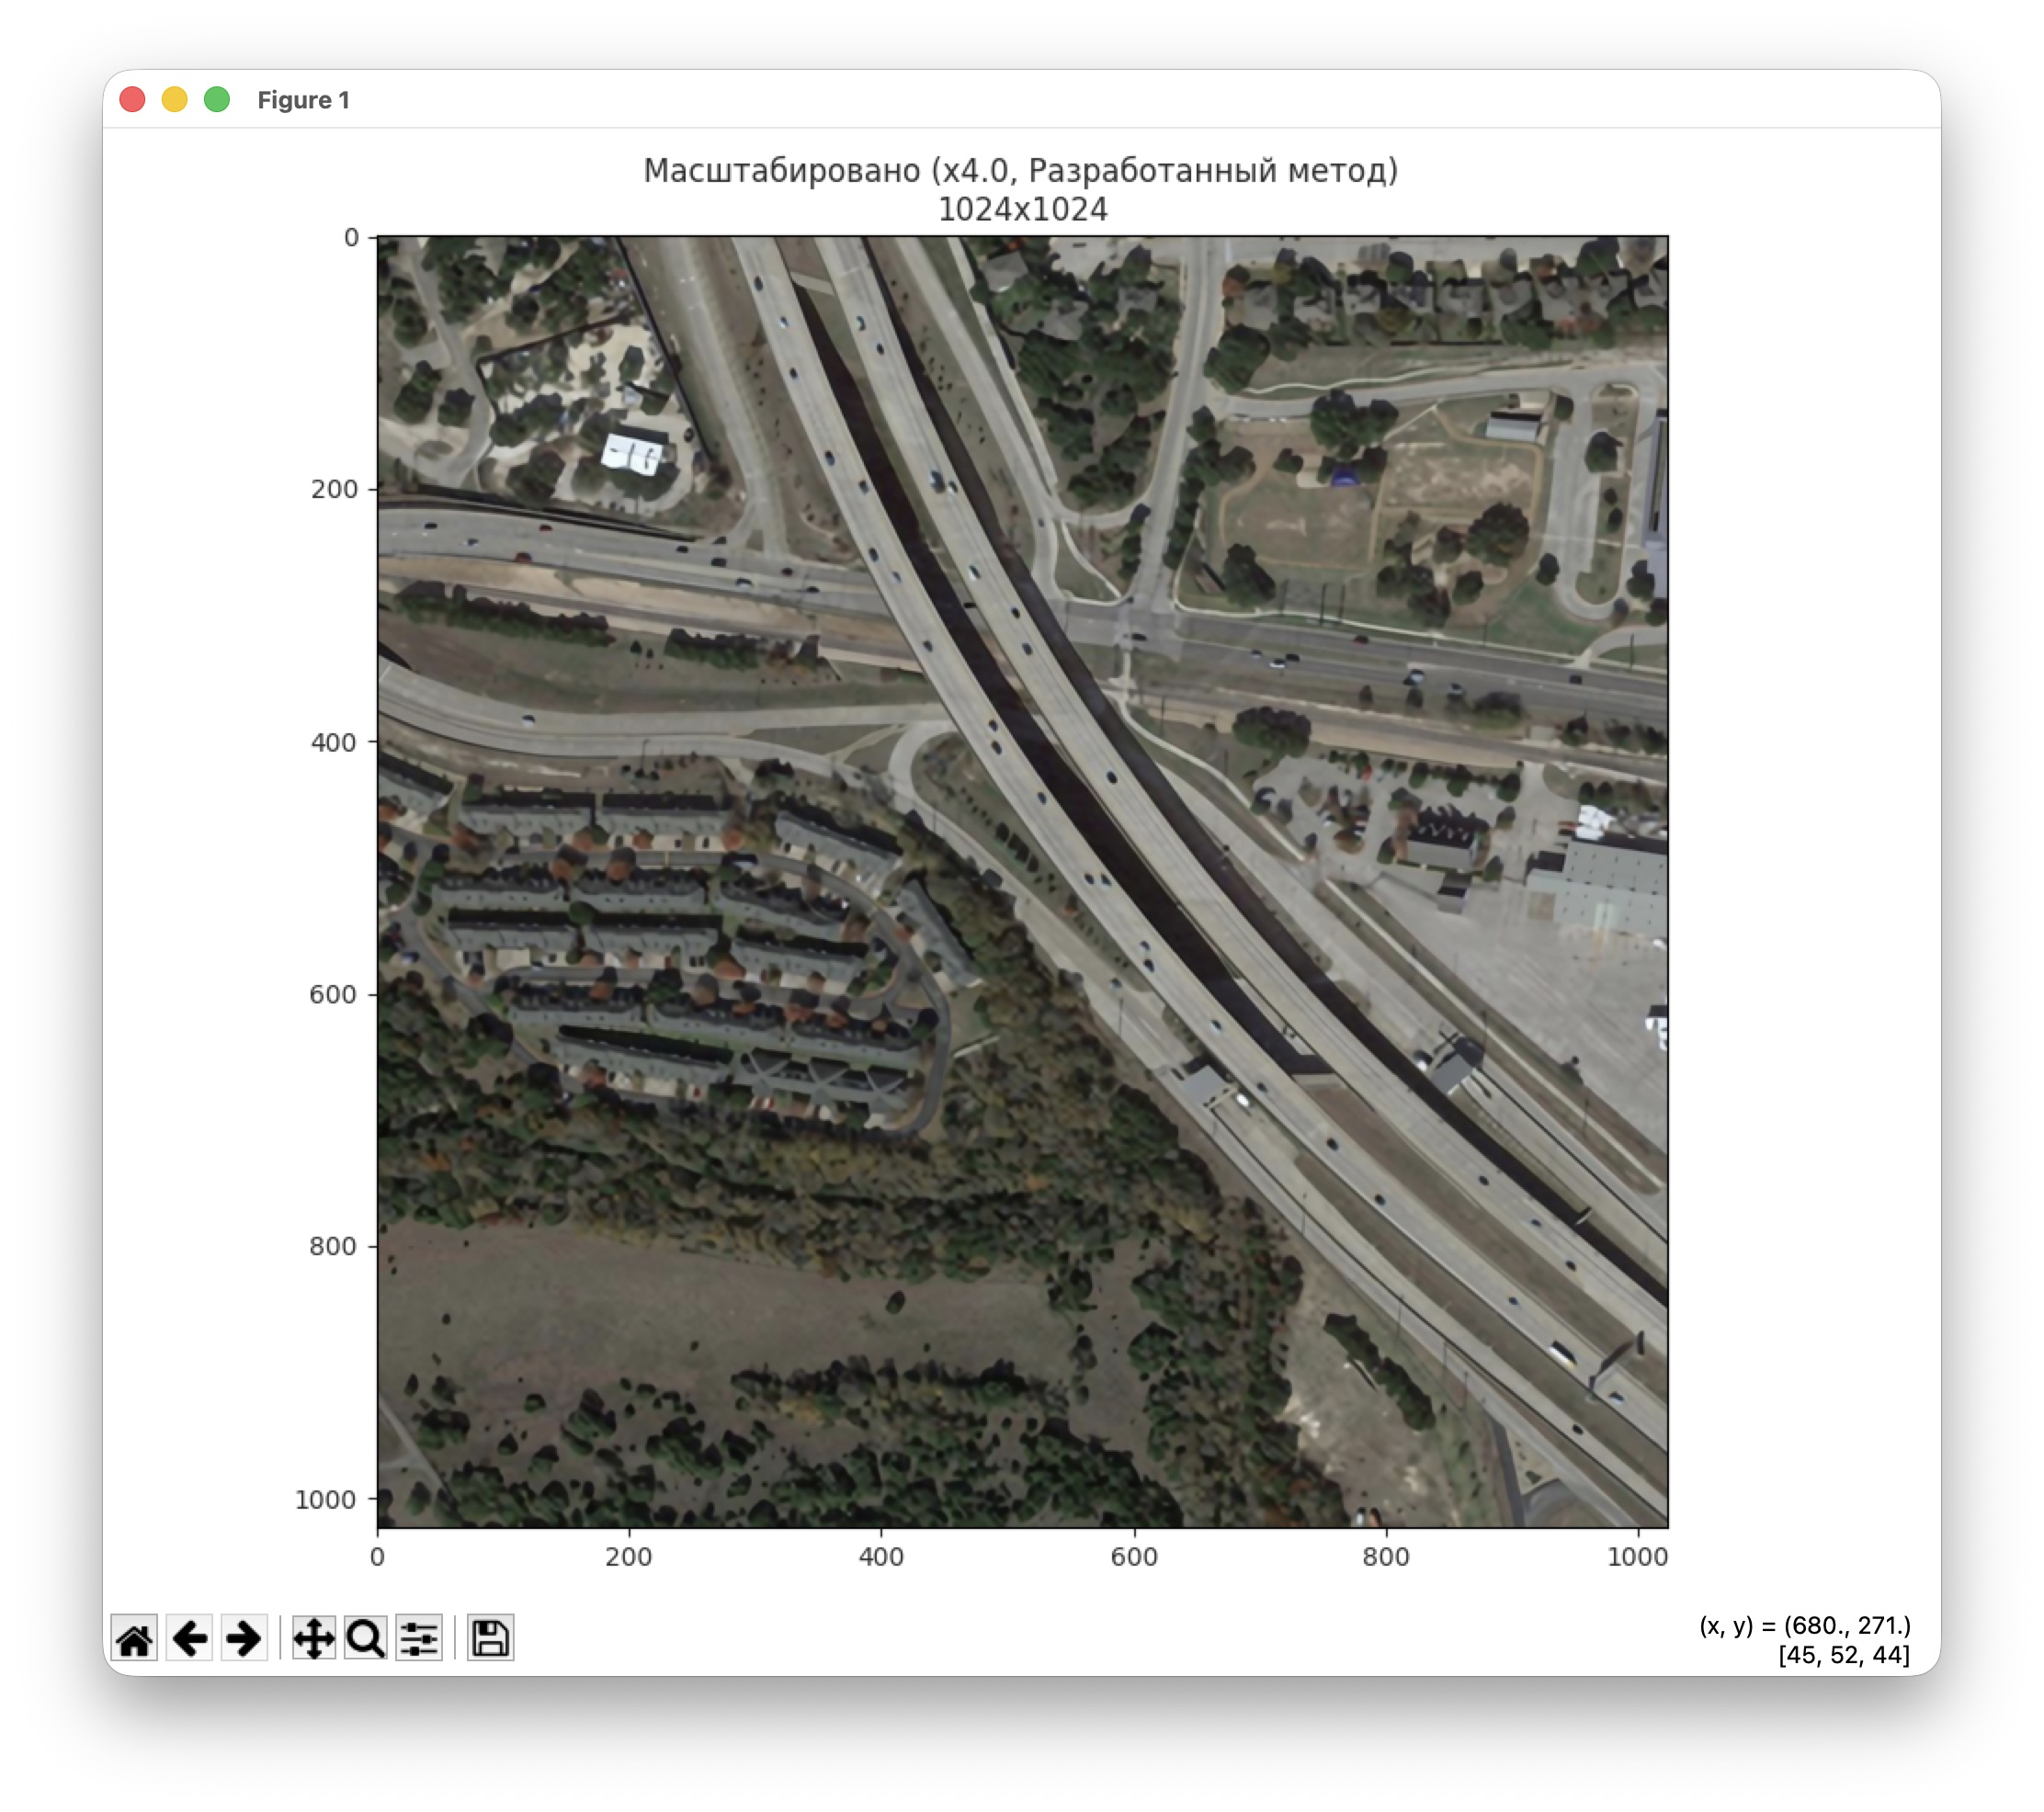
\includegraphics[width=0.6\linewidth]{images/technological/test_s1_out.jpeg}
    \caption{Изображение с разрешением $1024 \times 1024$ полученное масштабированием в 4 раза}
    \label{fig:tech:test_s1_out}
\end{figure}

\begin{figure}[H]
    \centering
    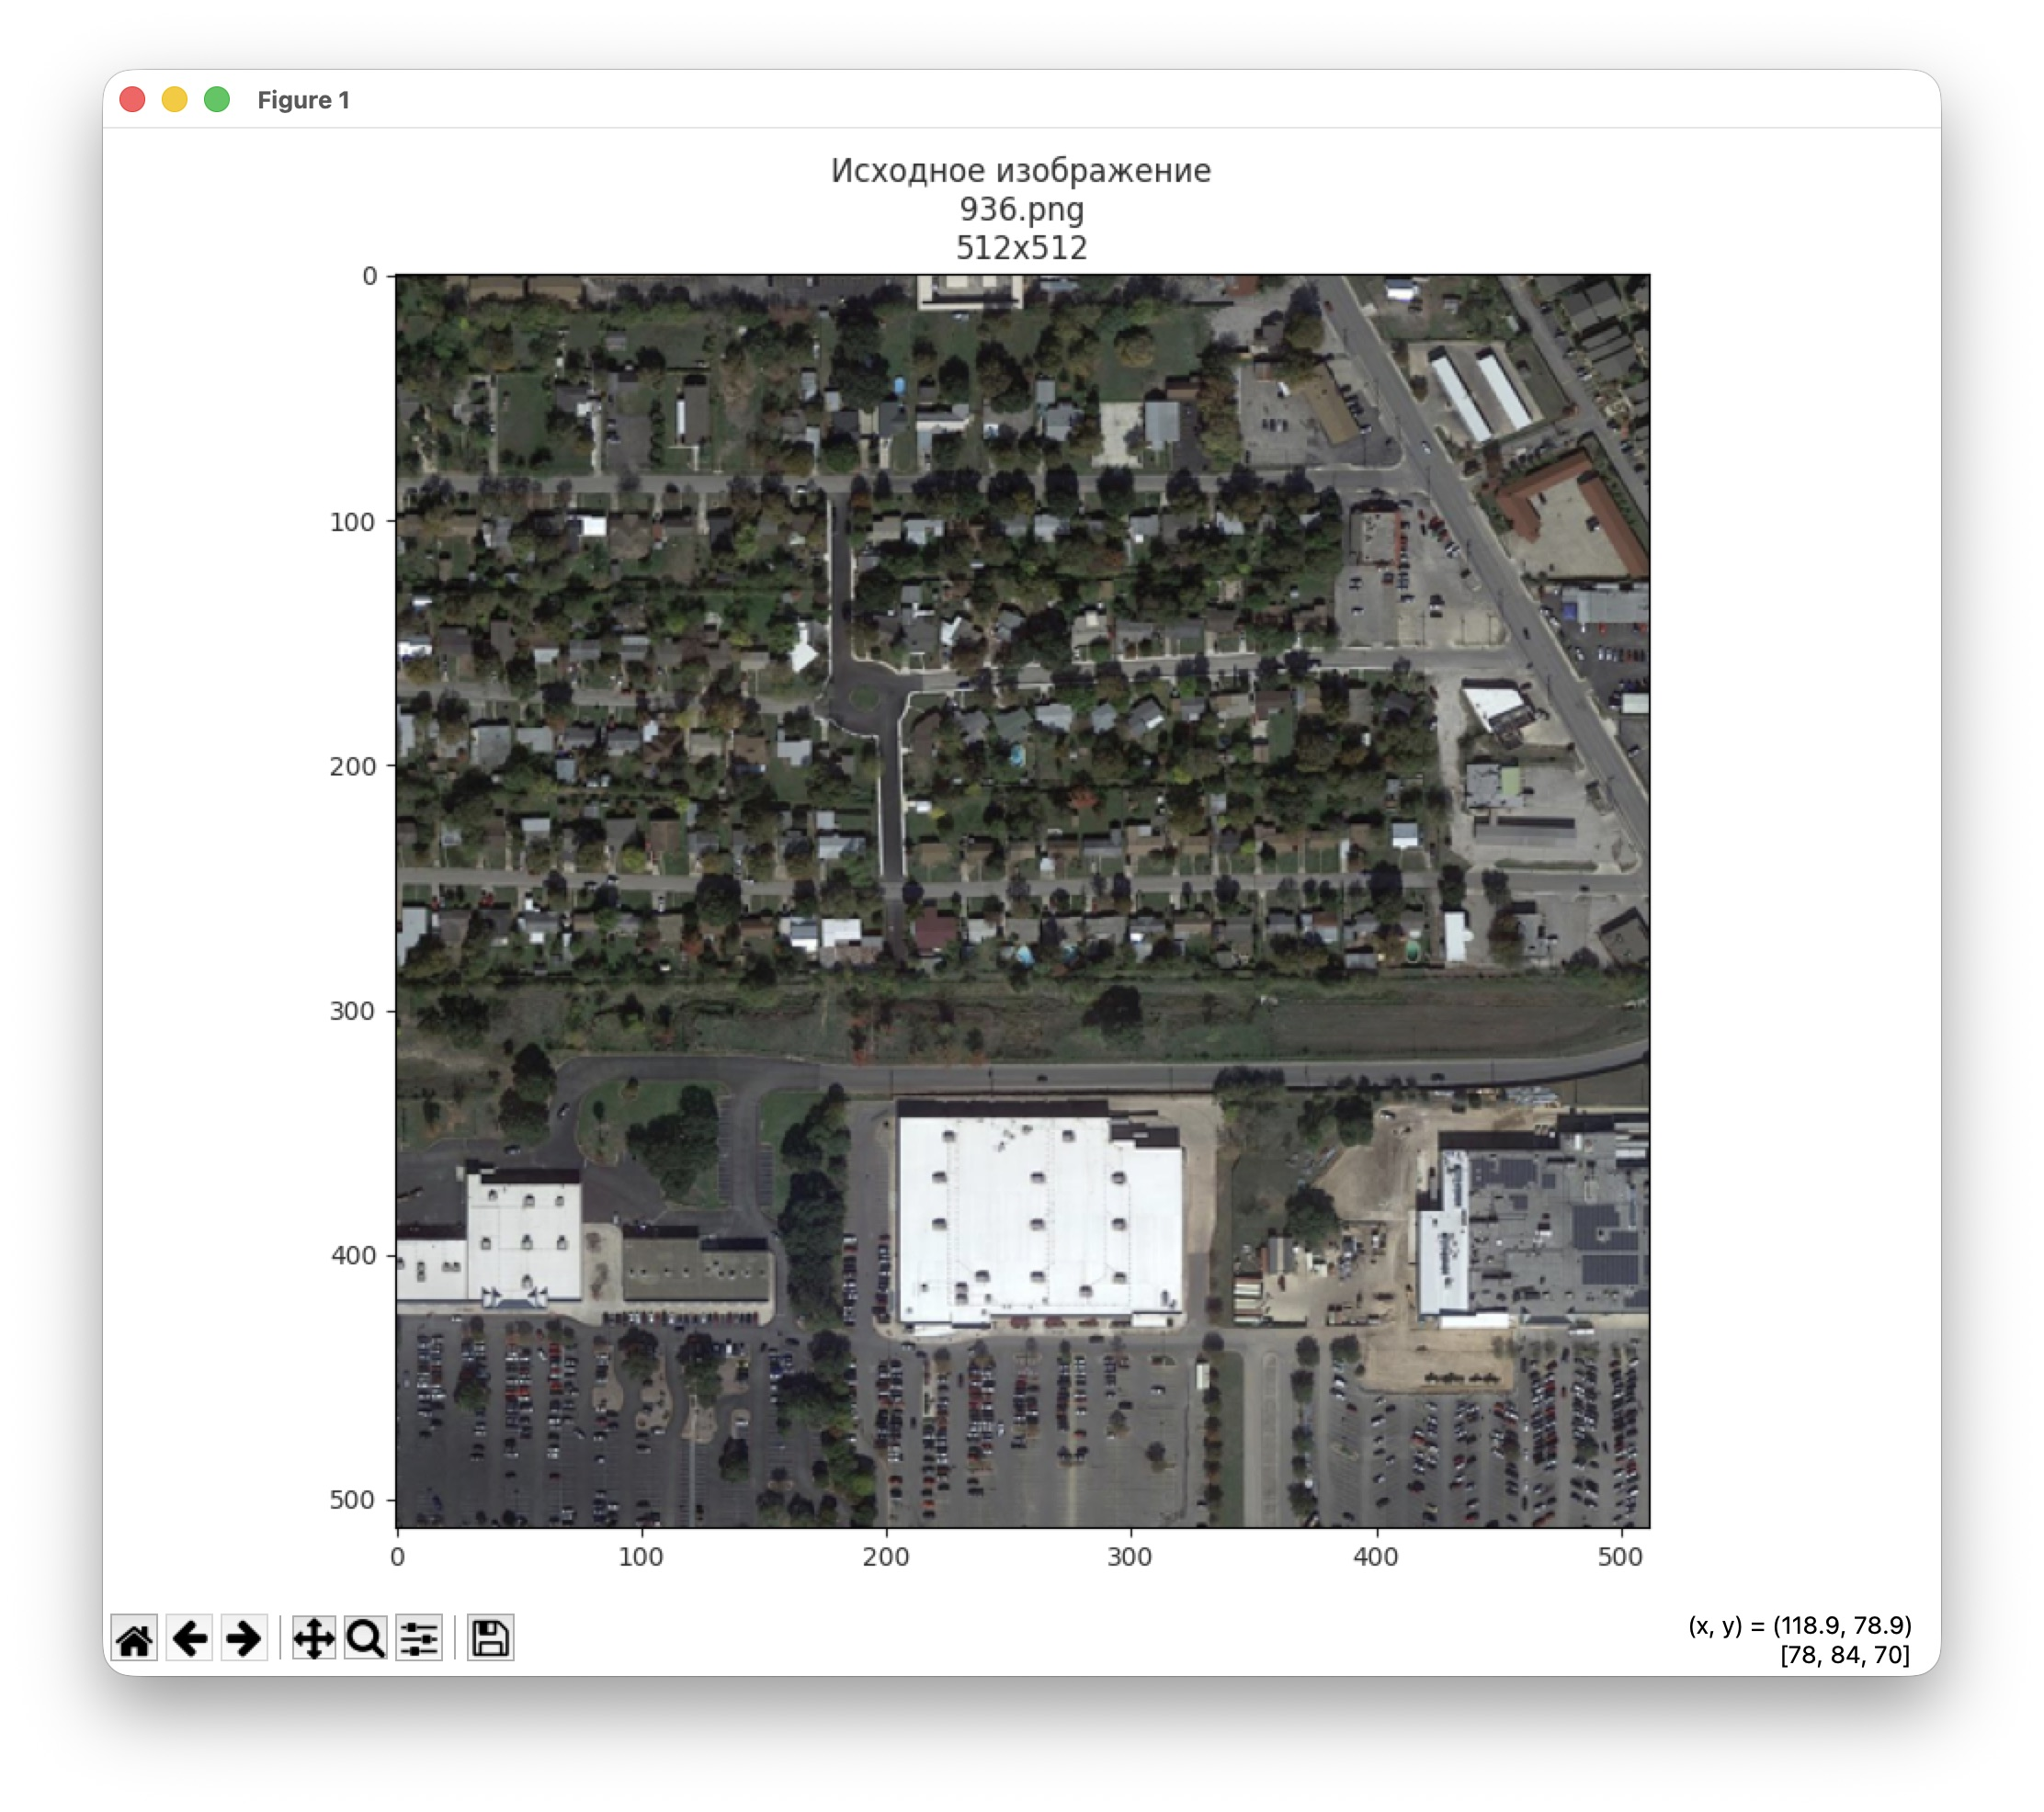
\includegraphics[width=0.6\linewidth]{images/technological/test_s2_in.jpeg}
    \caption{Входное изображение с разрешением $512 \times 512$}
    \label{fig:tech:test_s2_in}
\end{figure}

\begin{figure}[H]
    \centering
    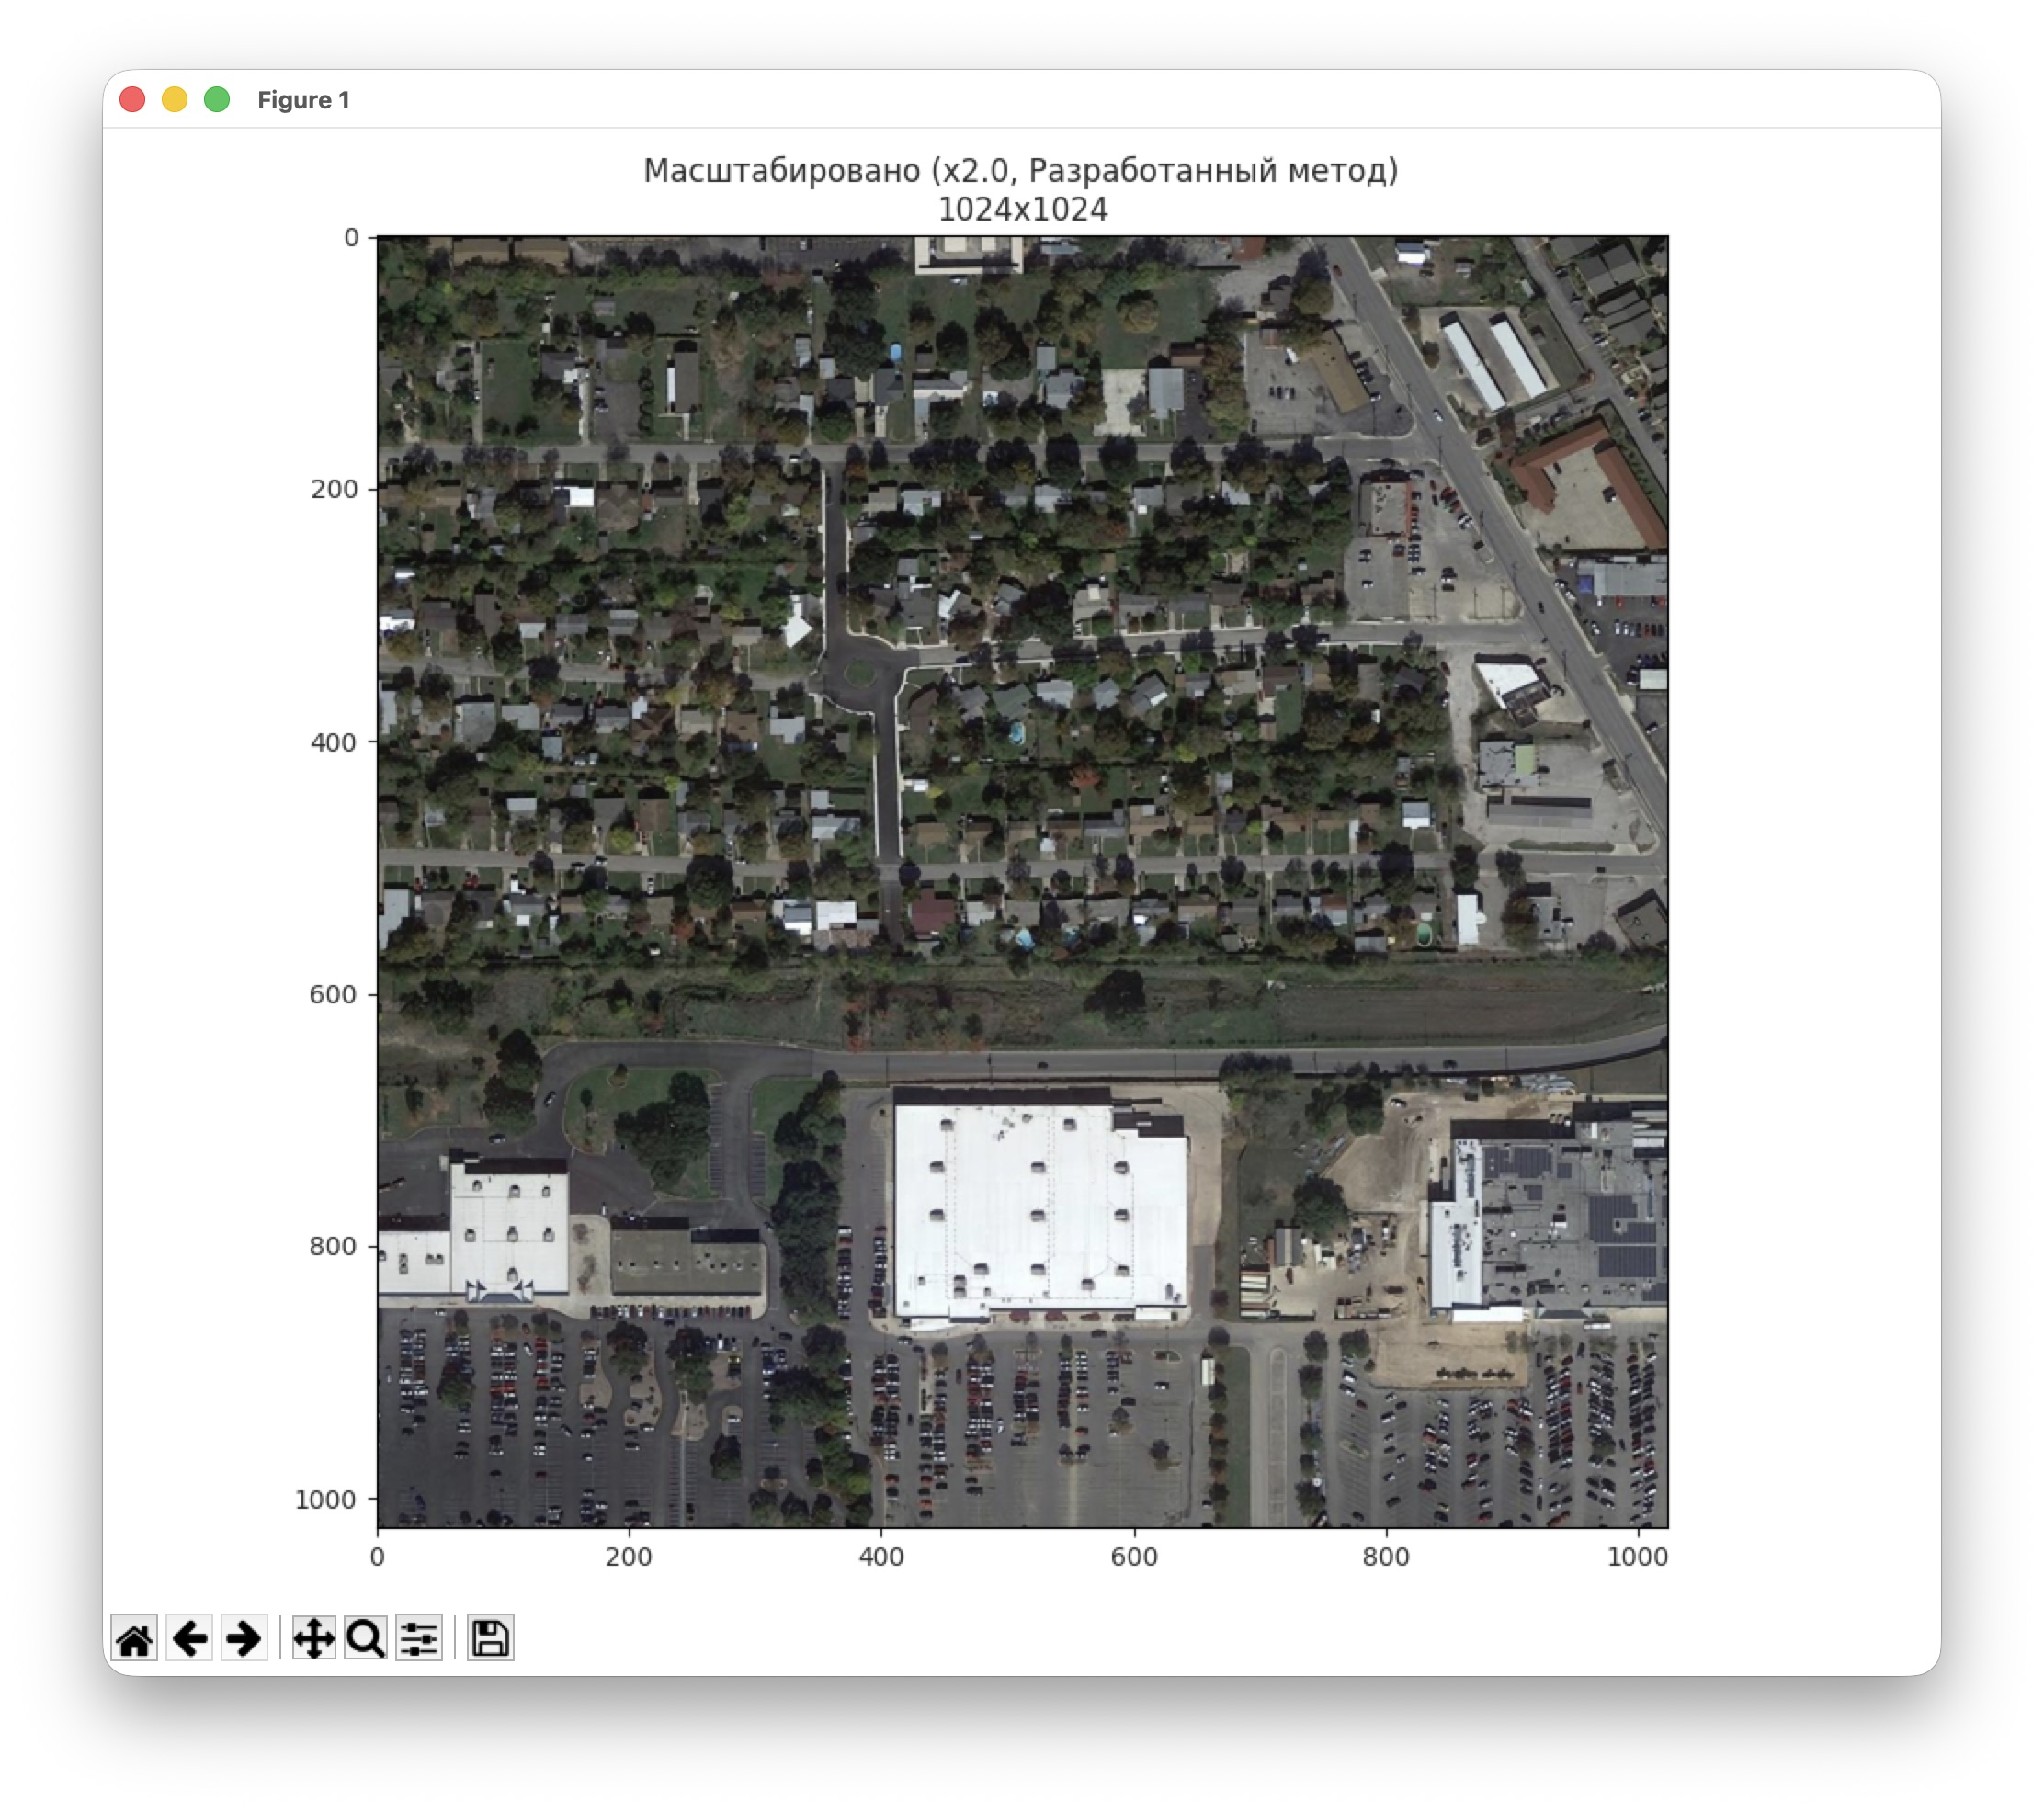
\includegraphics[width=0.6\linewidth]{images/technological/test_s2_out.jpeg}
    \caption{Изображение с разрешением $1024 \times 1024$ полученное масштабированием в 2 раза}
    \label{fig:tech:test_s2_out}
\end{figure}

\begin{figure}[H]
    \centering
    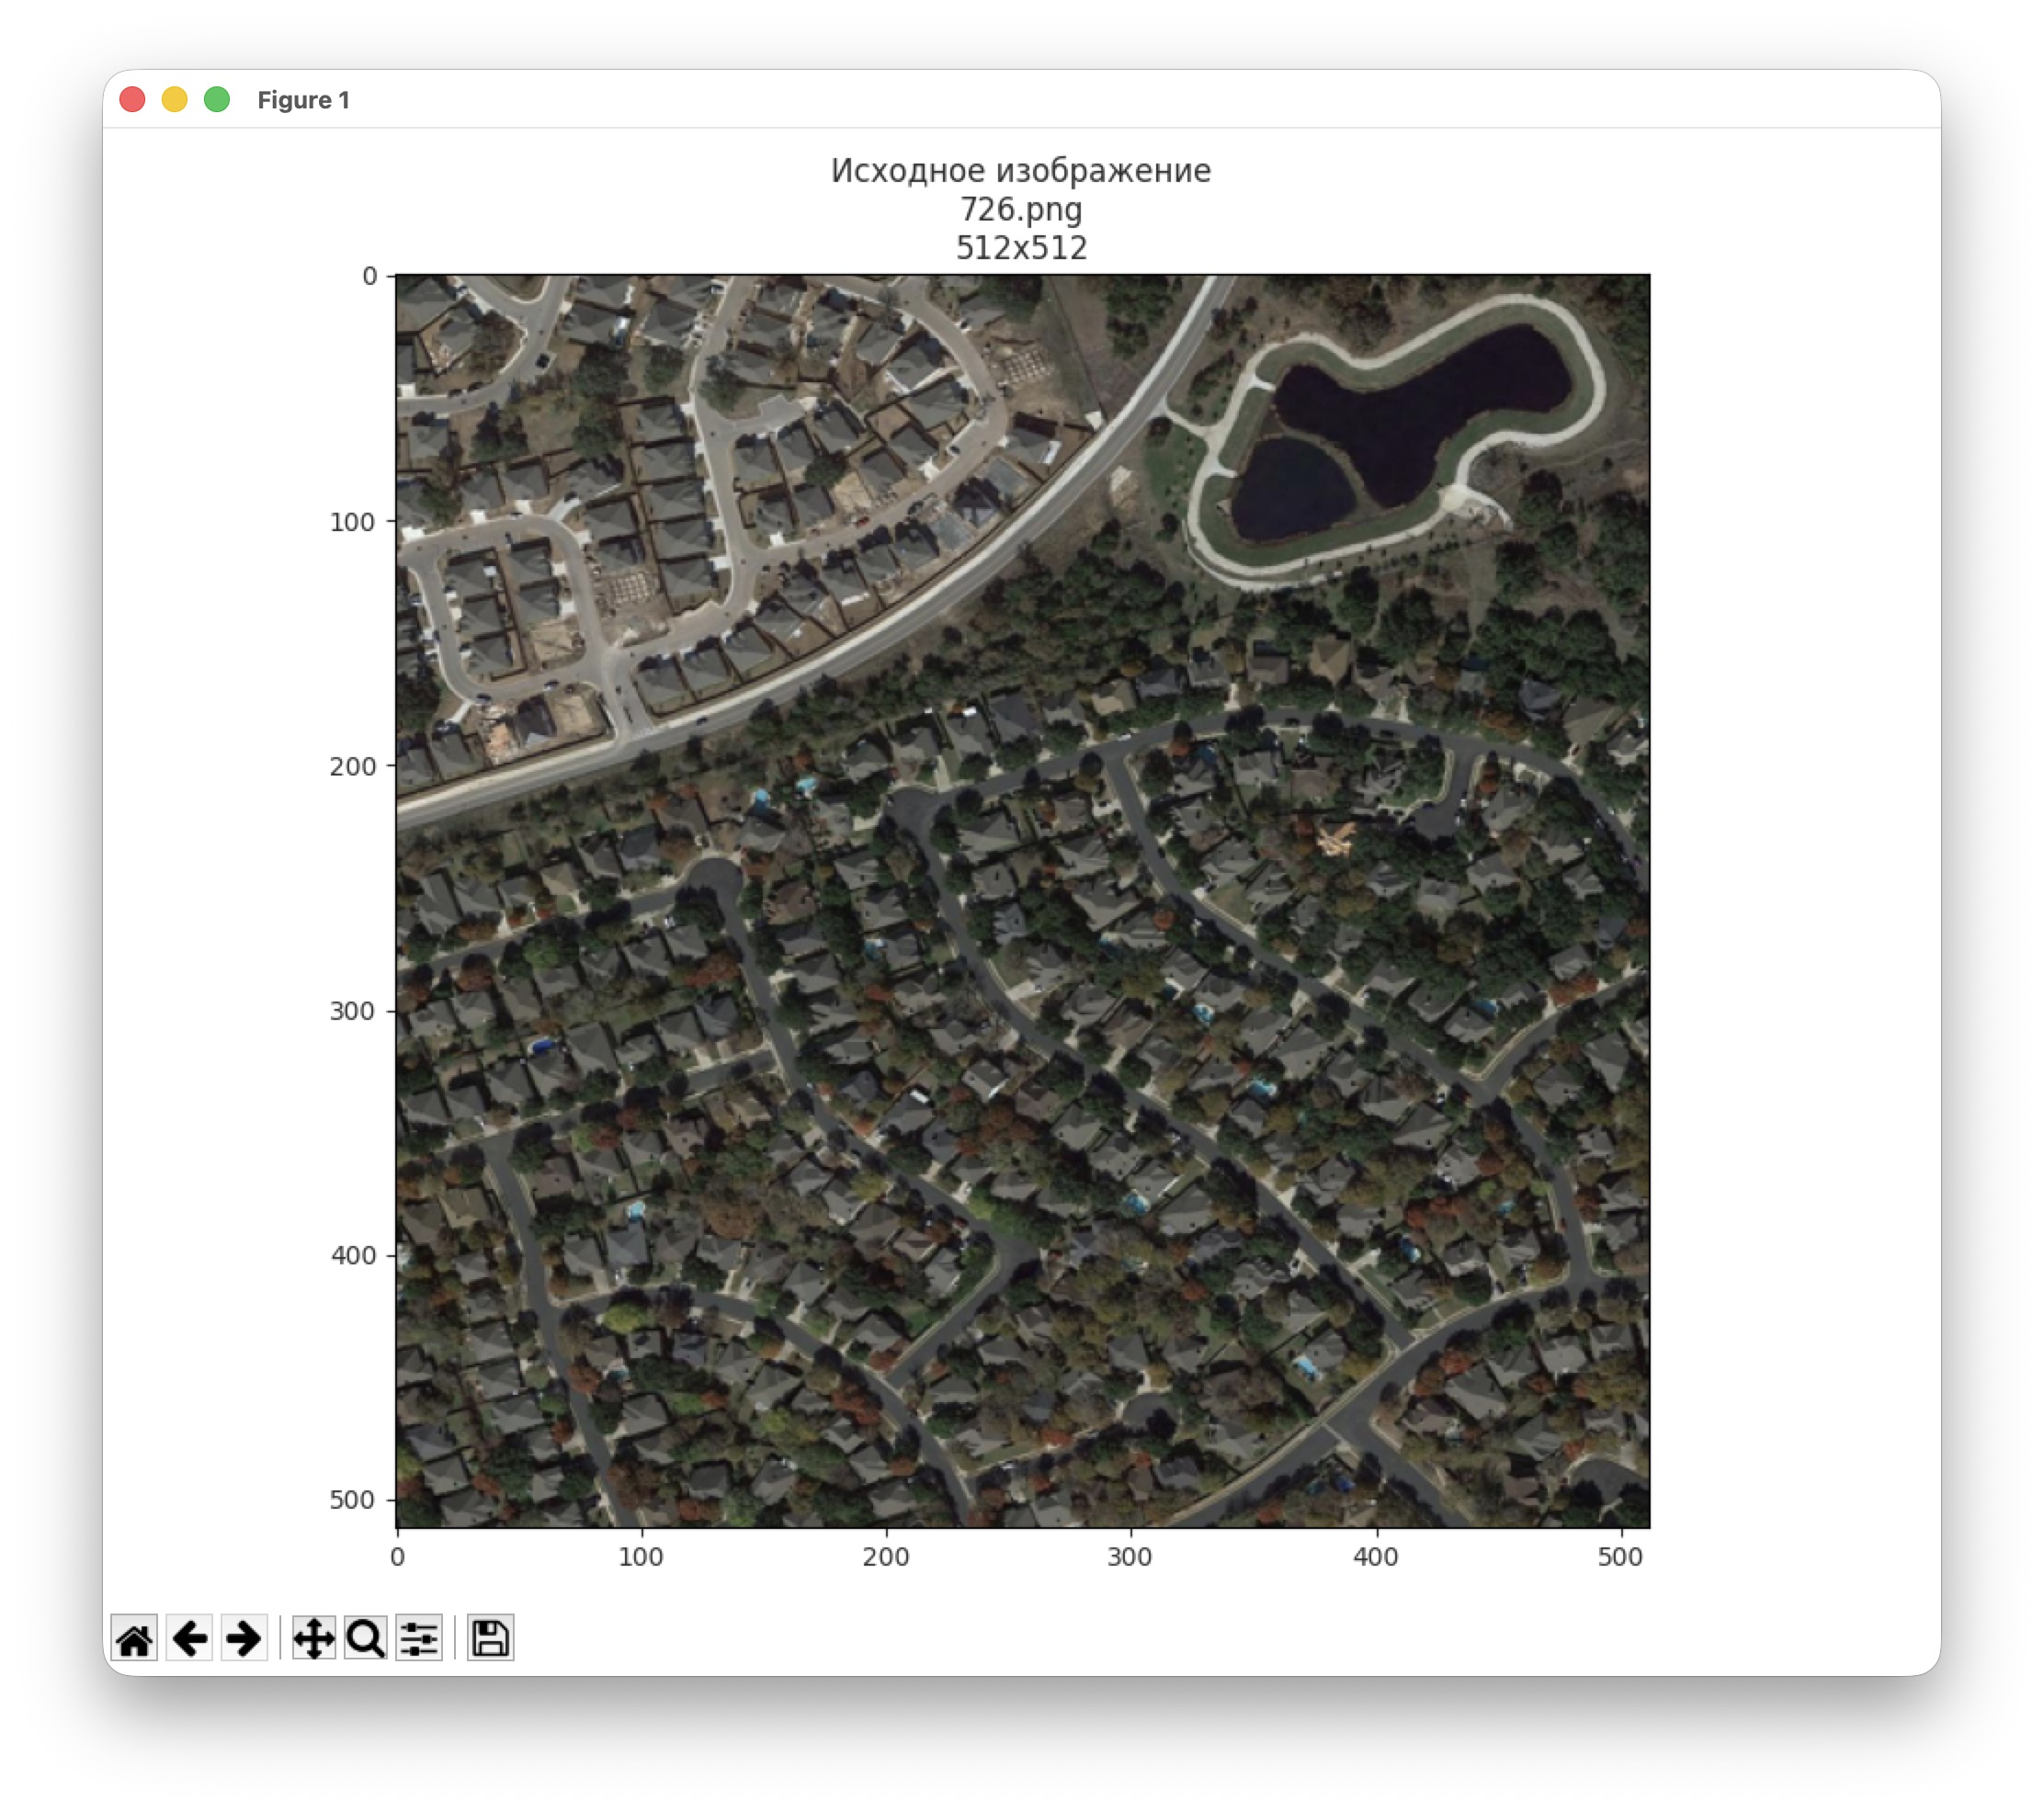
\includegraphics[width=0.6\linewidth]{images/technological/test_s3_in.jpeg}
    \caption{Входное изображение с разрешением $512 \times 512$}
    \label{fig:tech:test_s3_in}
\end{figure}

\begin{figure}[H]
    \centering
    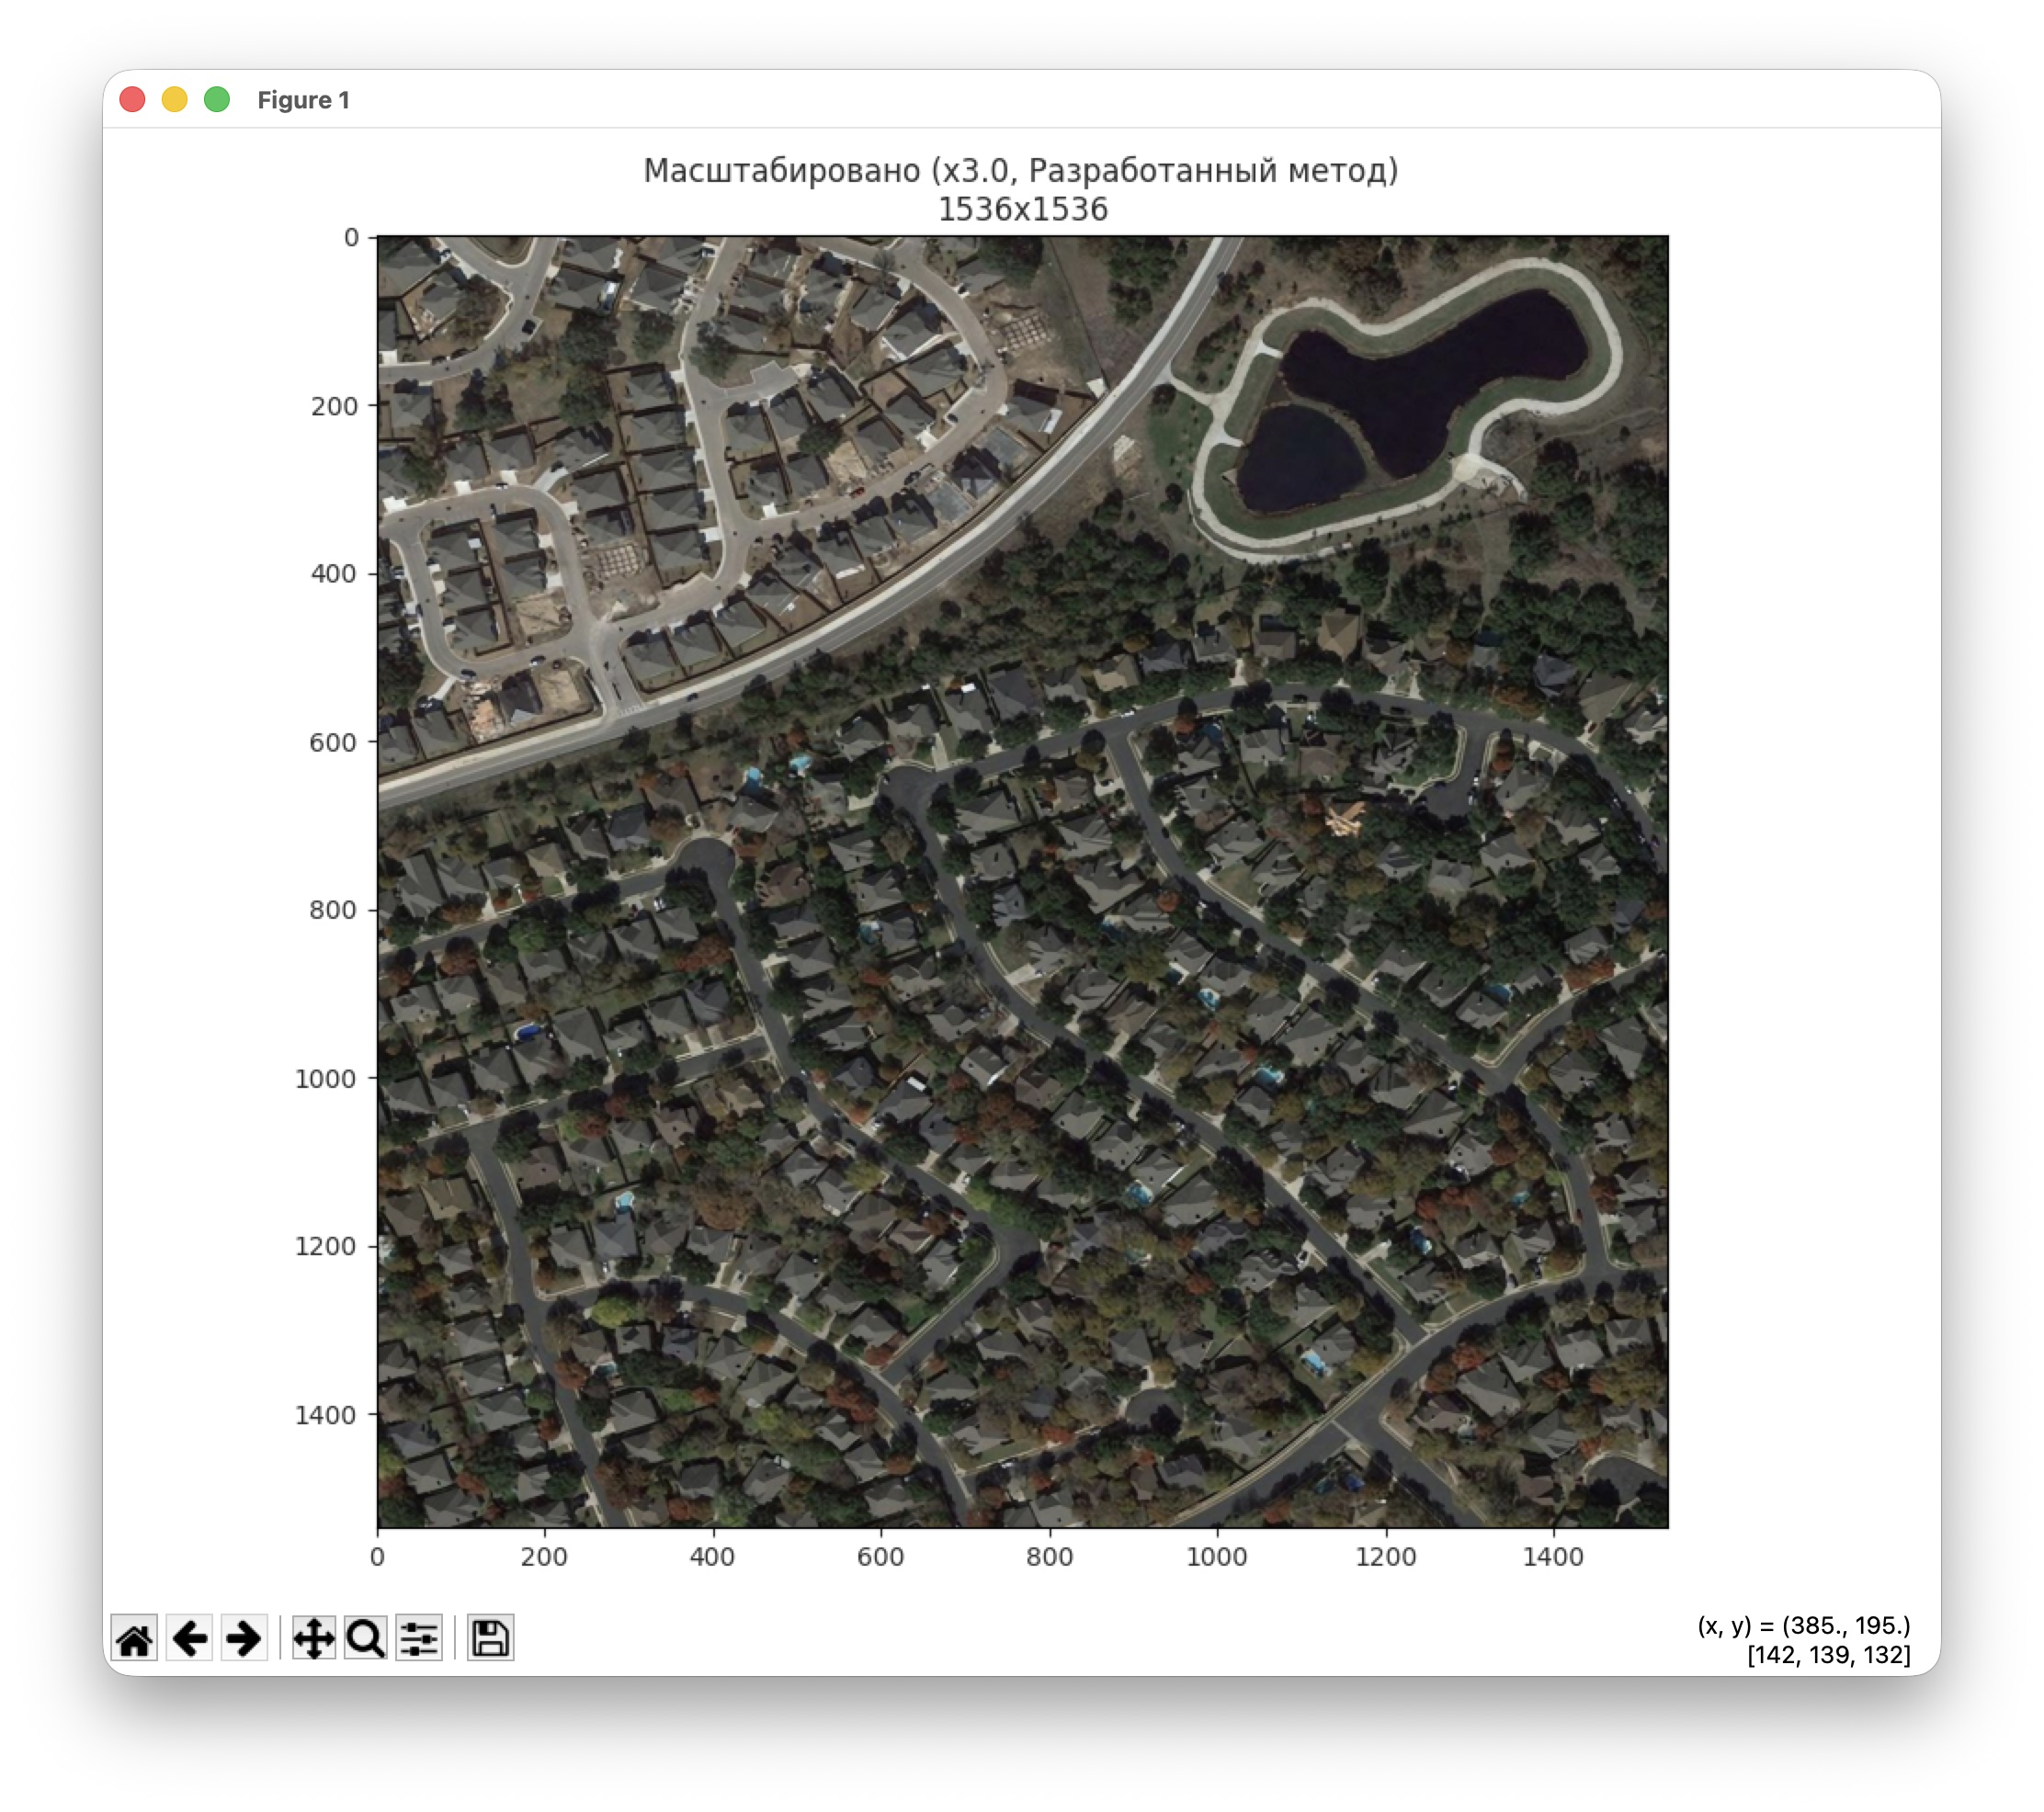
\includegraphics[width=0.6\linewidth]{images/technological/test_s3_out.jpeg}
    \caption{Изображение с разрешением $1536 \times 1536$ полученное масштабированием в 3 раза}
    \label{fig:tech:test_s3_out}
\end{figure}

\begin{figure}[H]
    \centering
    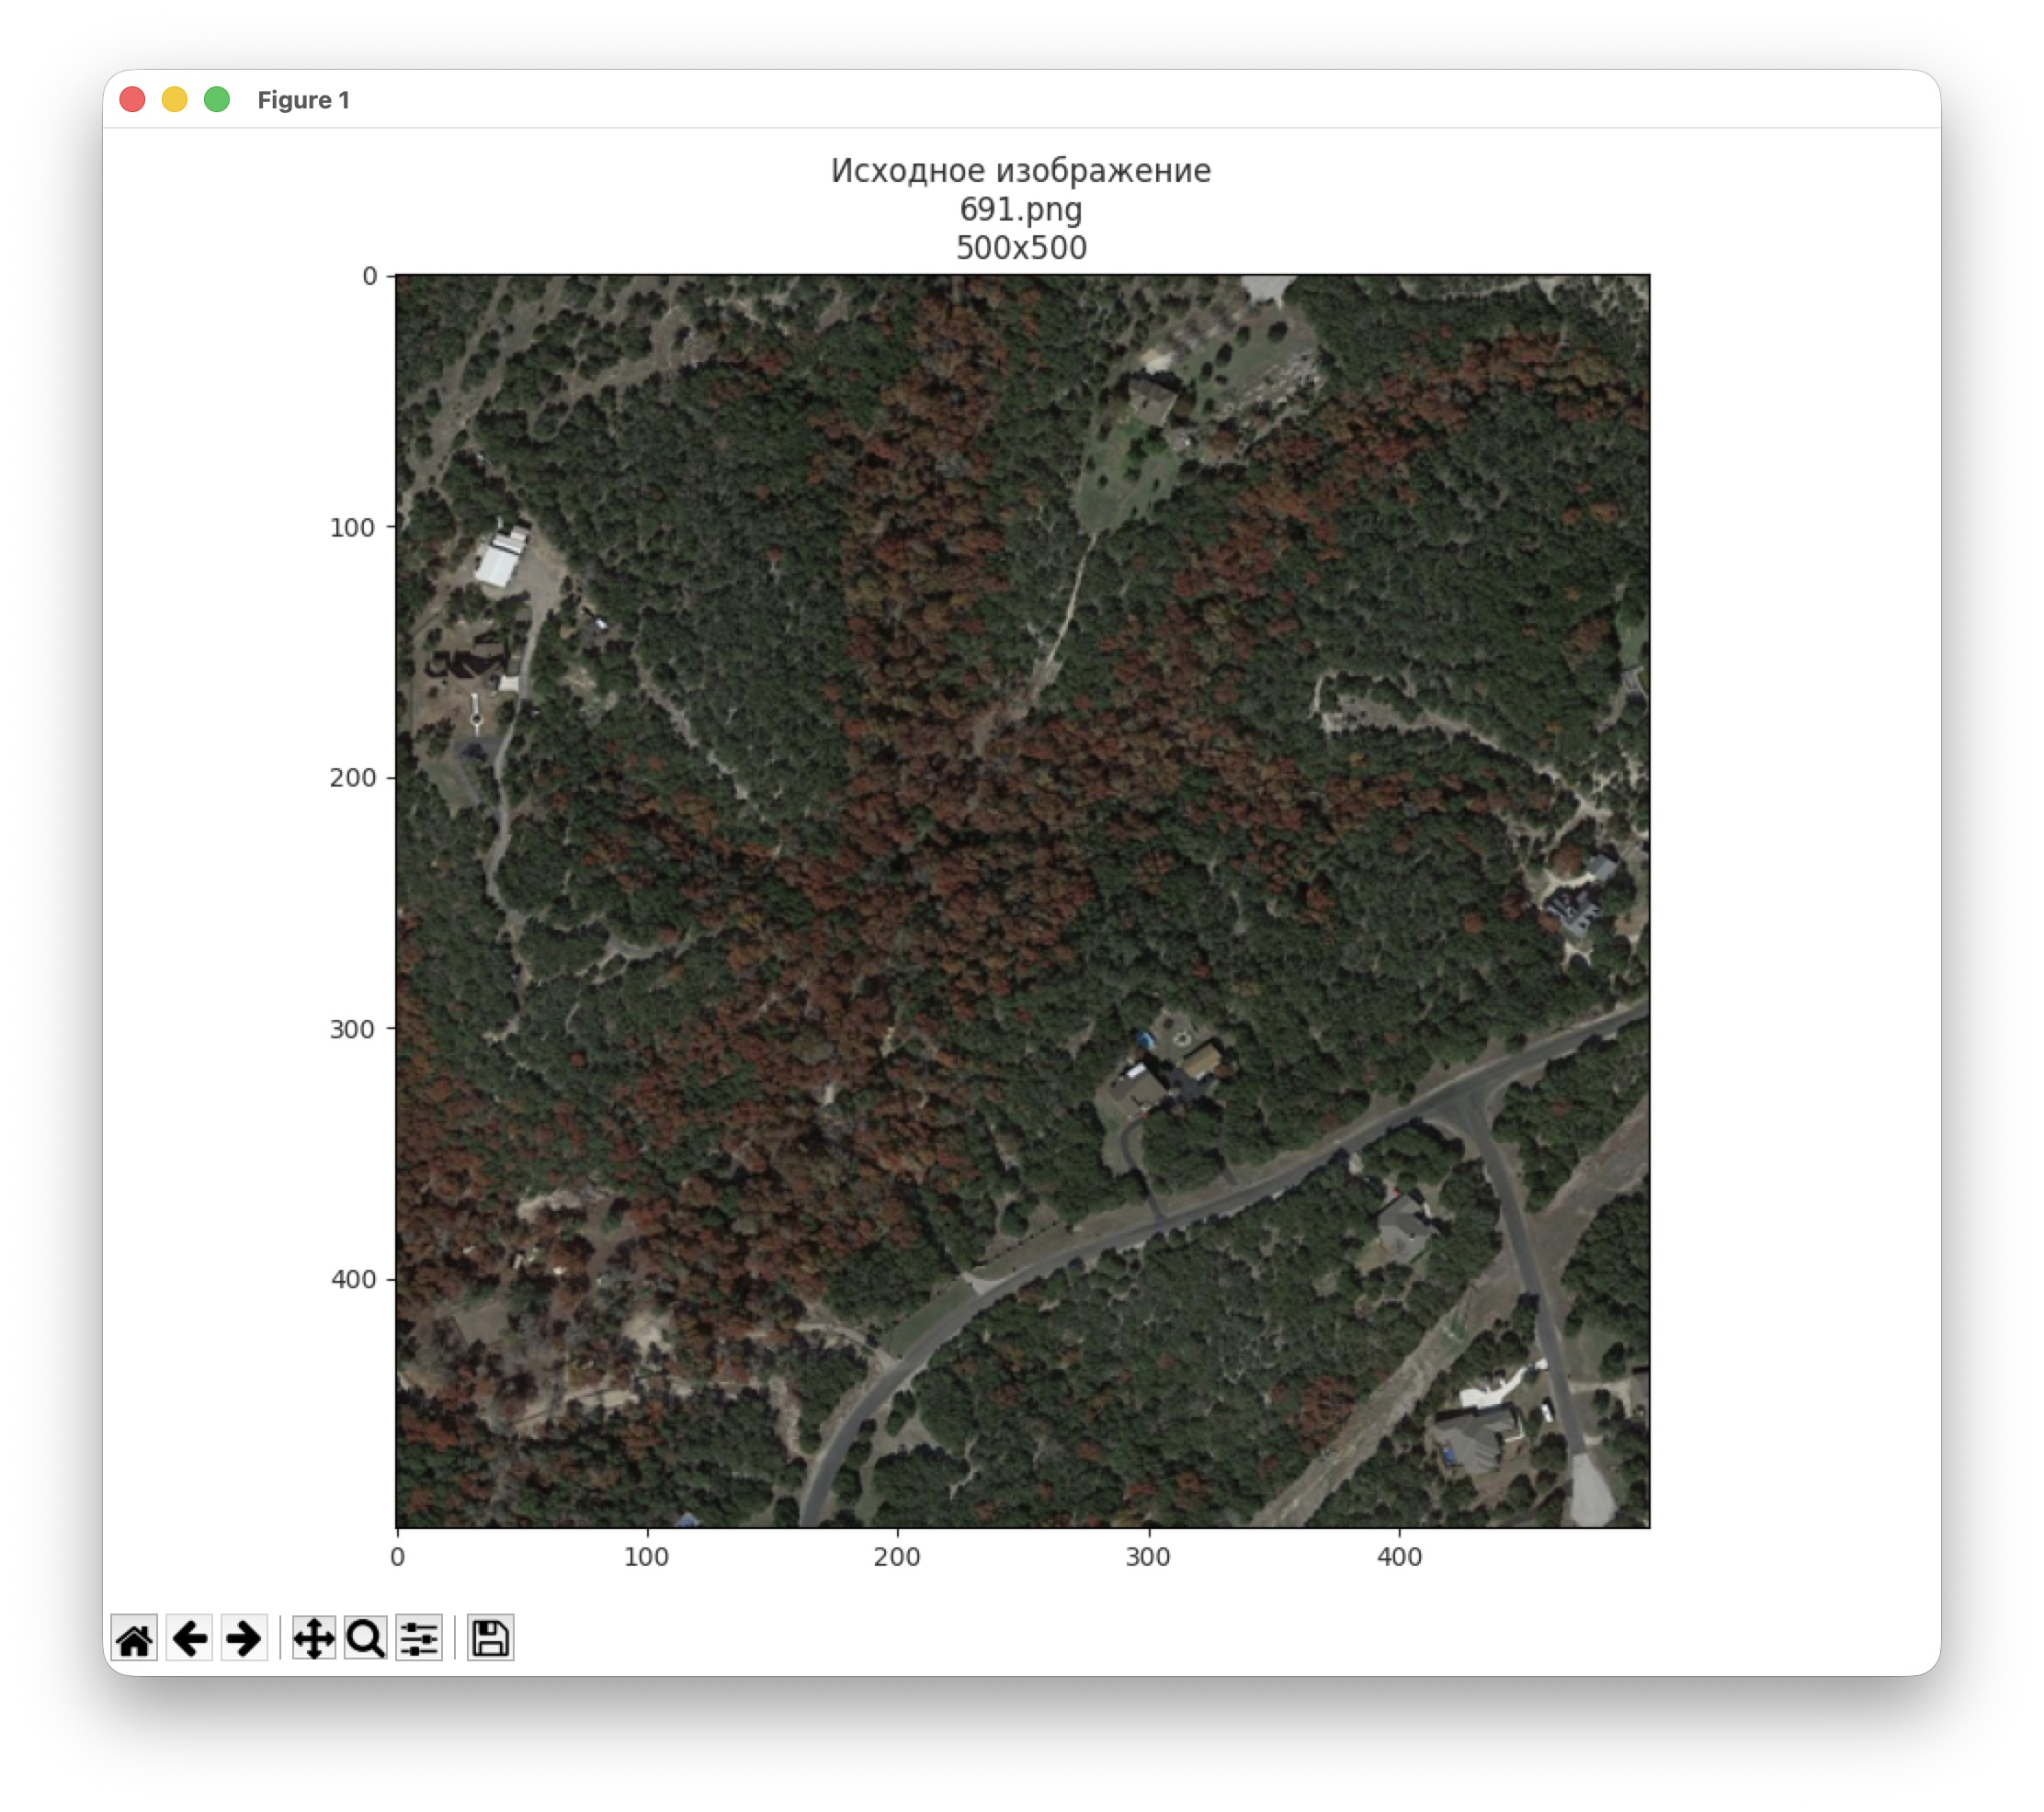
\includegraphics[width=0.6\linewidth]{images/technological/test_s4_in.jpeg}
    \caption{Входное изображение с разрешением $500 \times 500$}
    \label{fig:tech:test_s4_in}
\end{figure}

\begin{figure}[H]
    \centering
    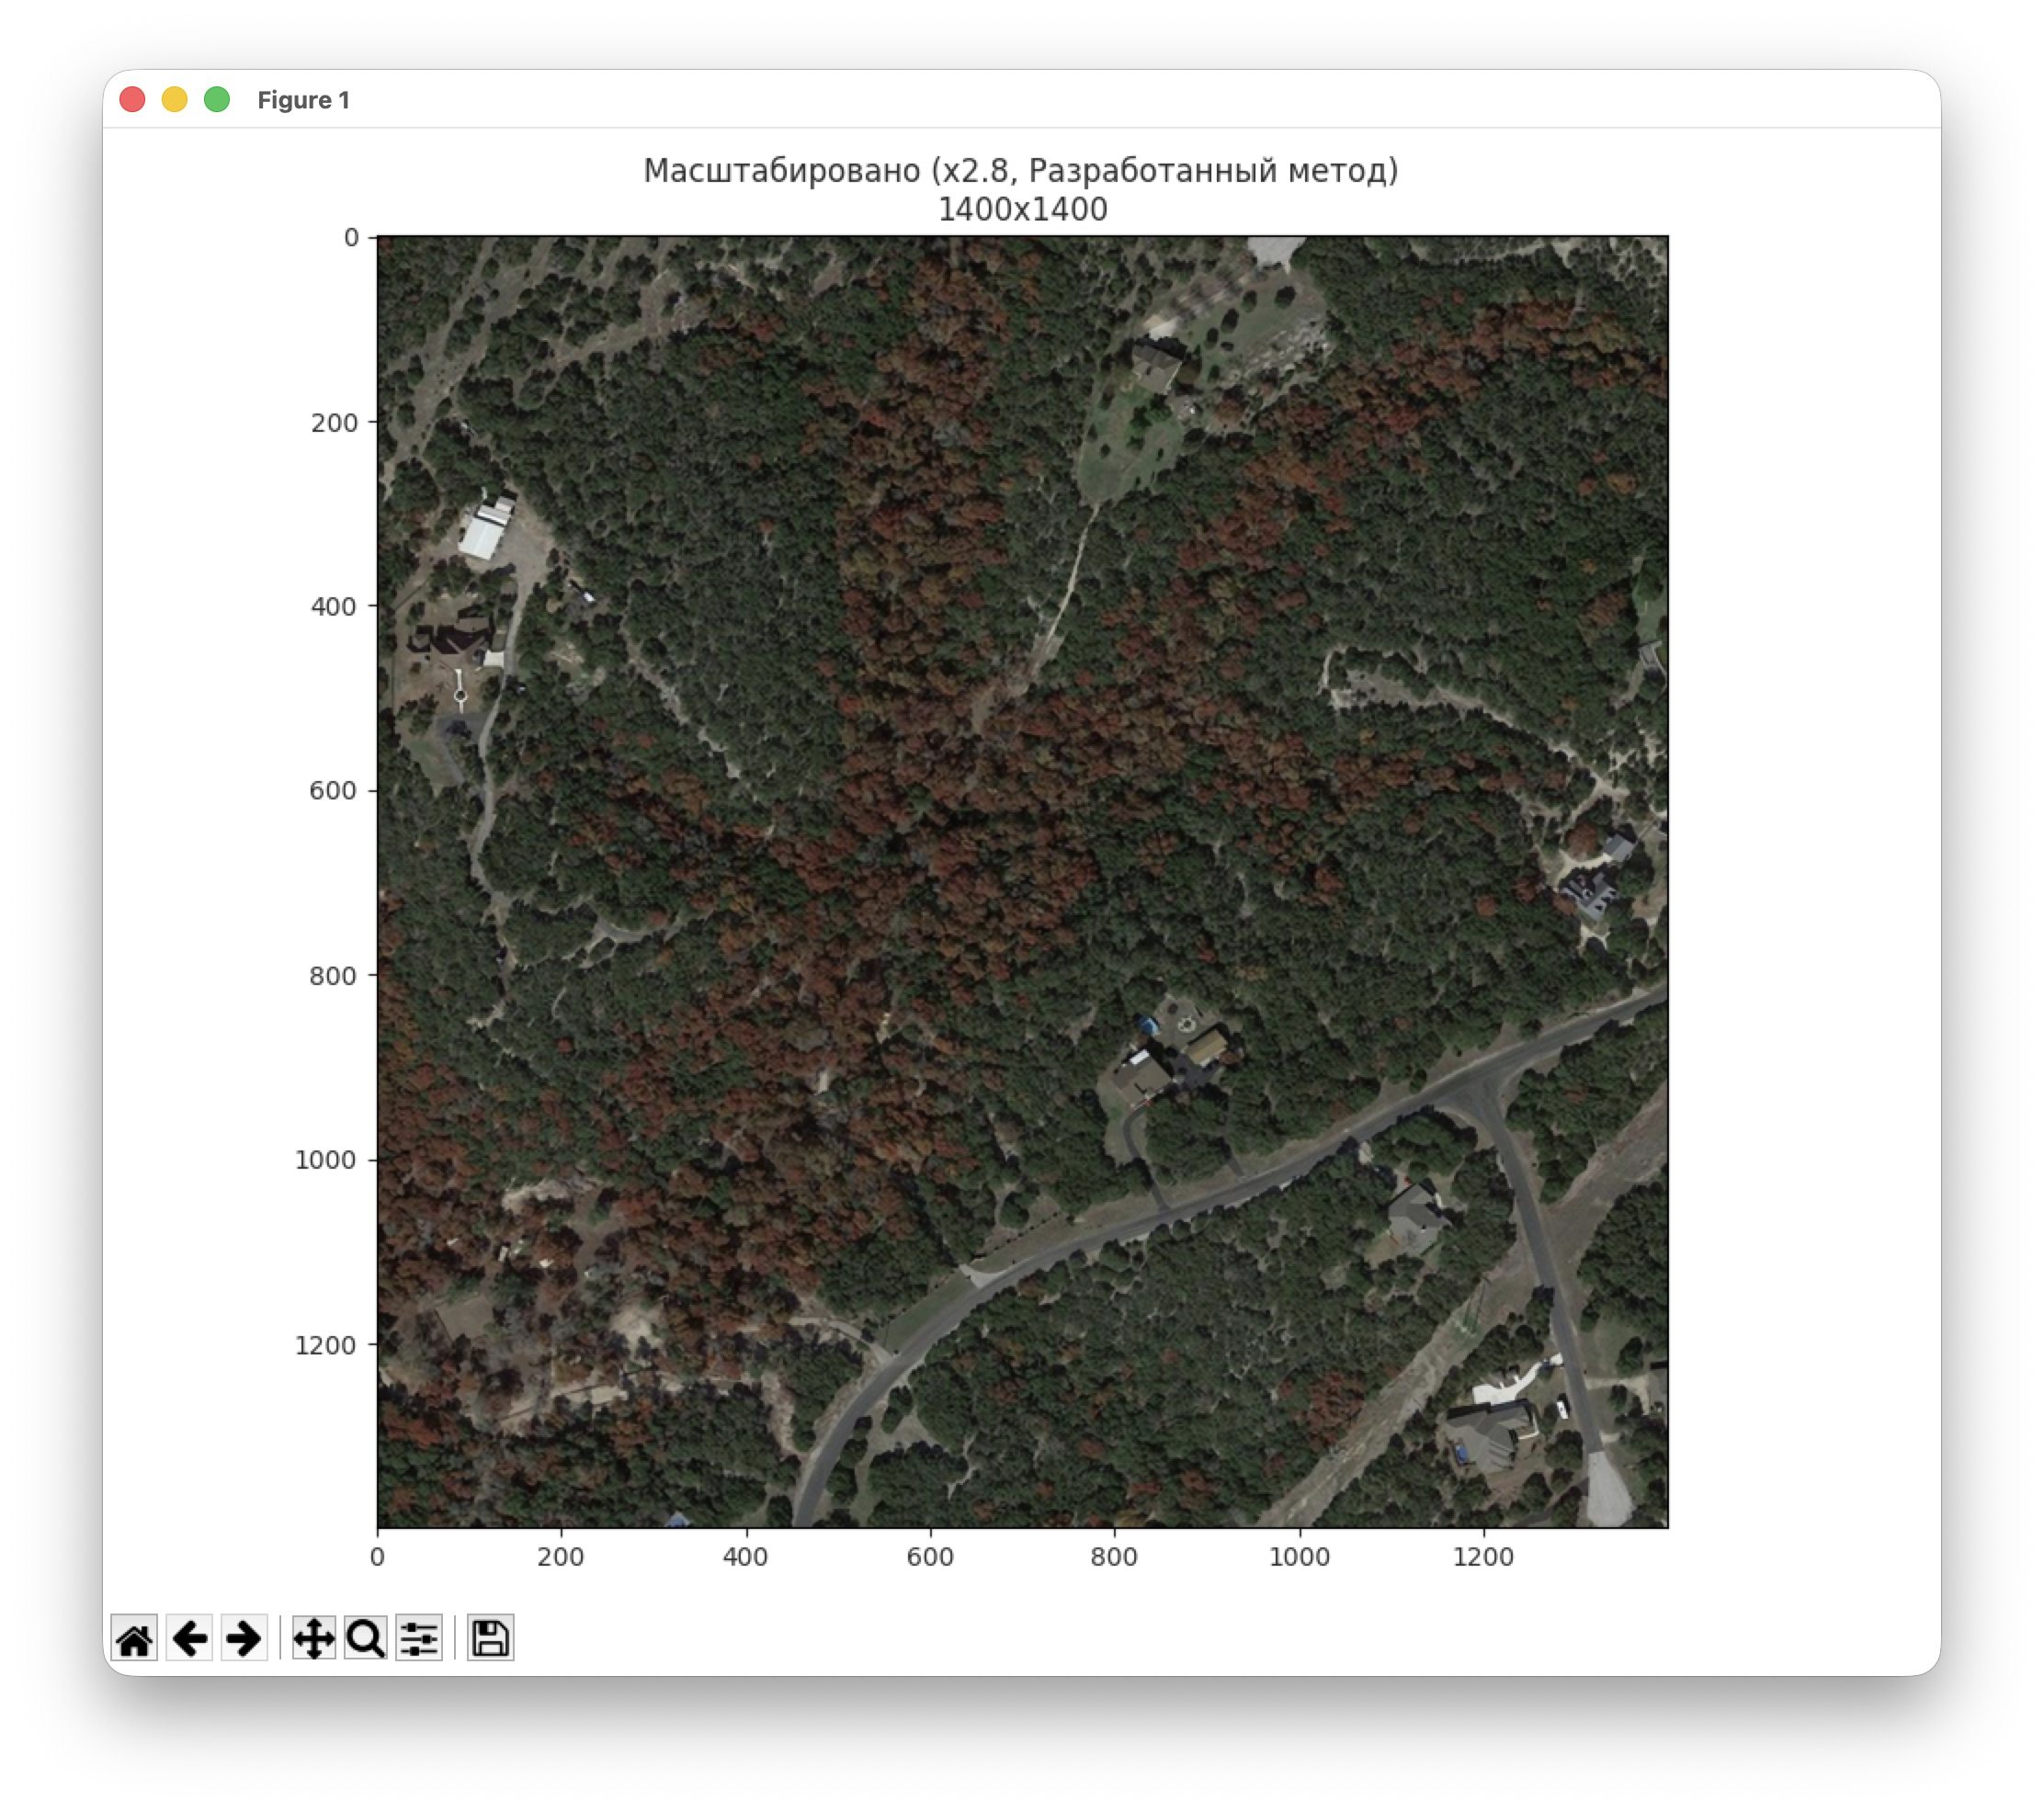
\includegraphics[width=0.6\linewidth]{images/technological/test_s4_out.jpeg}
    \caption{Изображение с разрешением $1400 \times 1400$ полученное масштабированием в 2.8 раз}
    \label{fig:tech:test_s4_out}
\end{figure}

\begin{figure}[H]
    \centering
    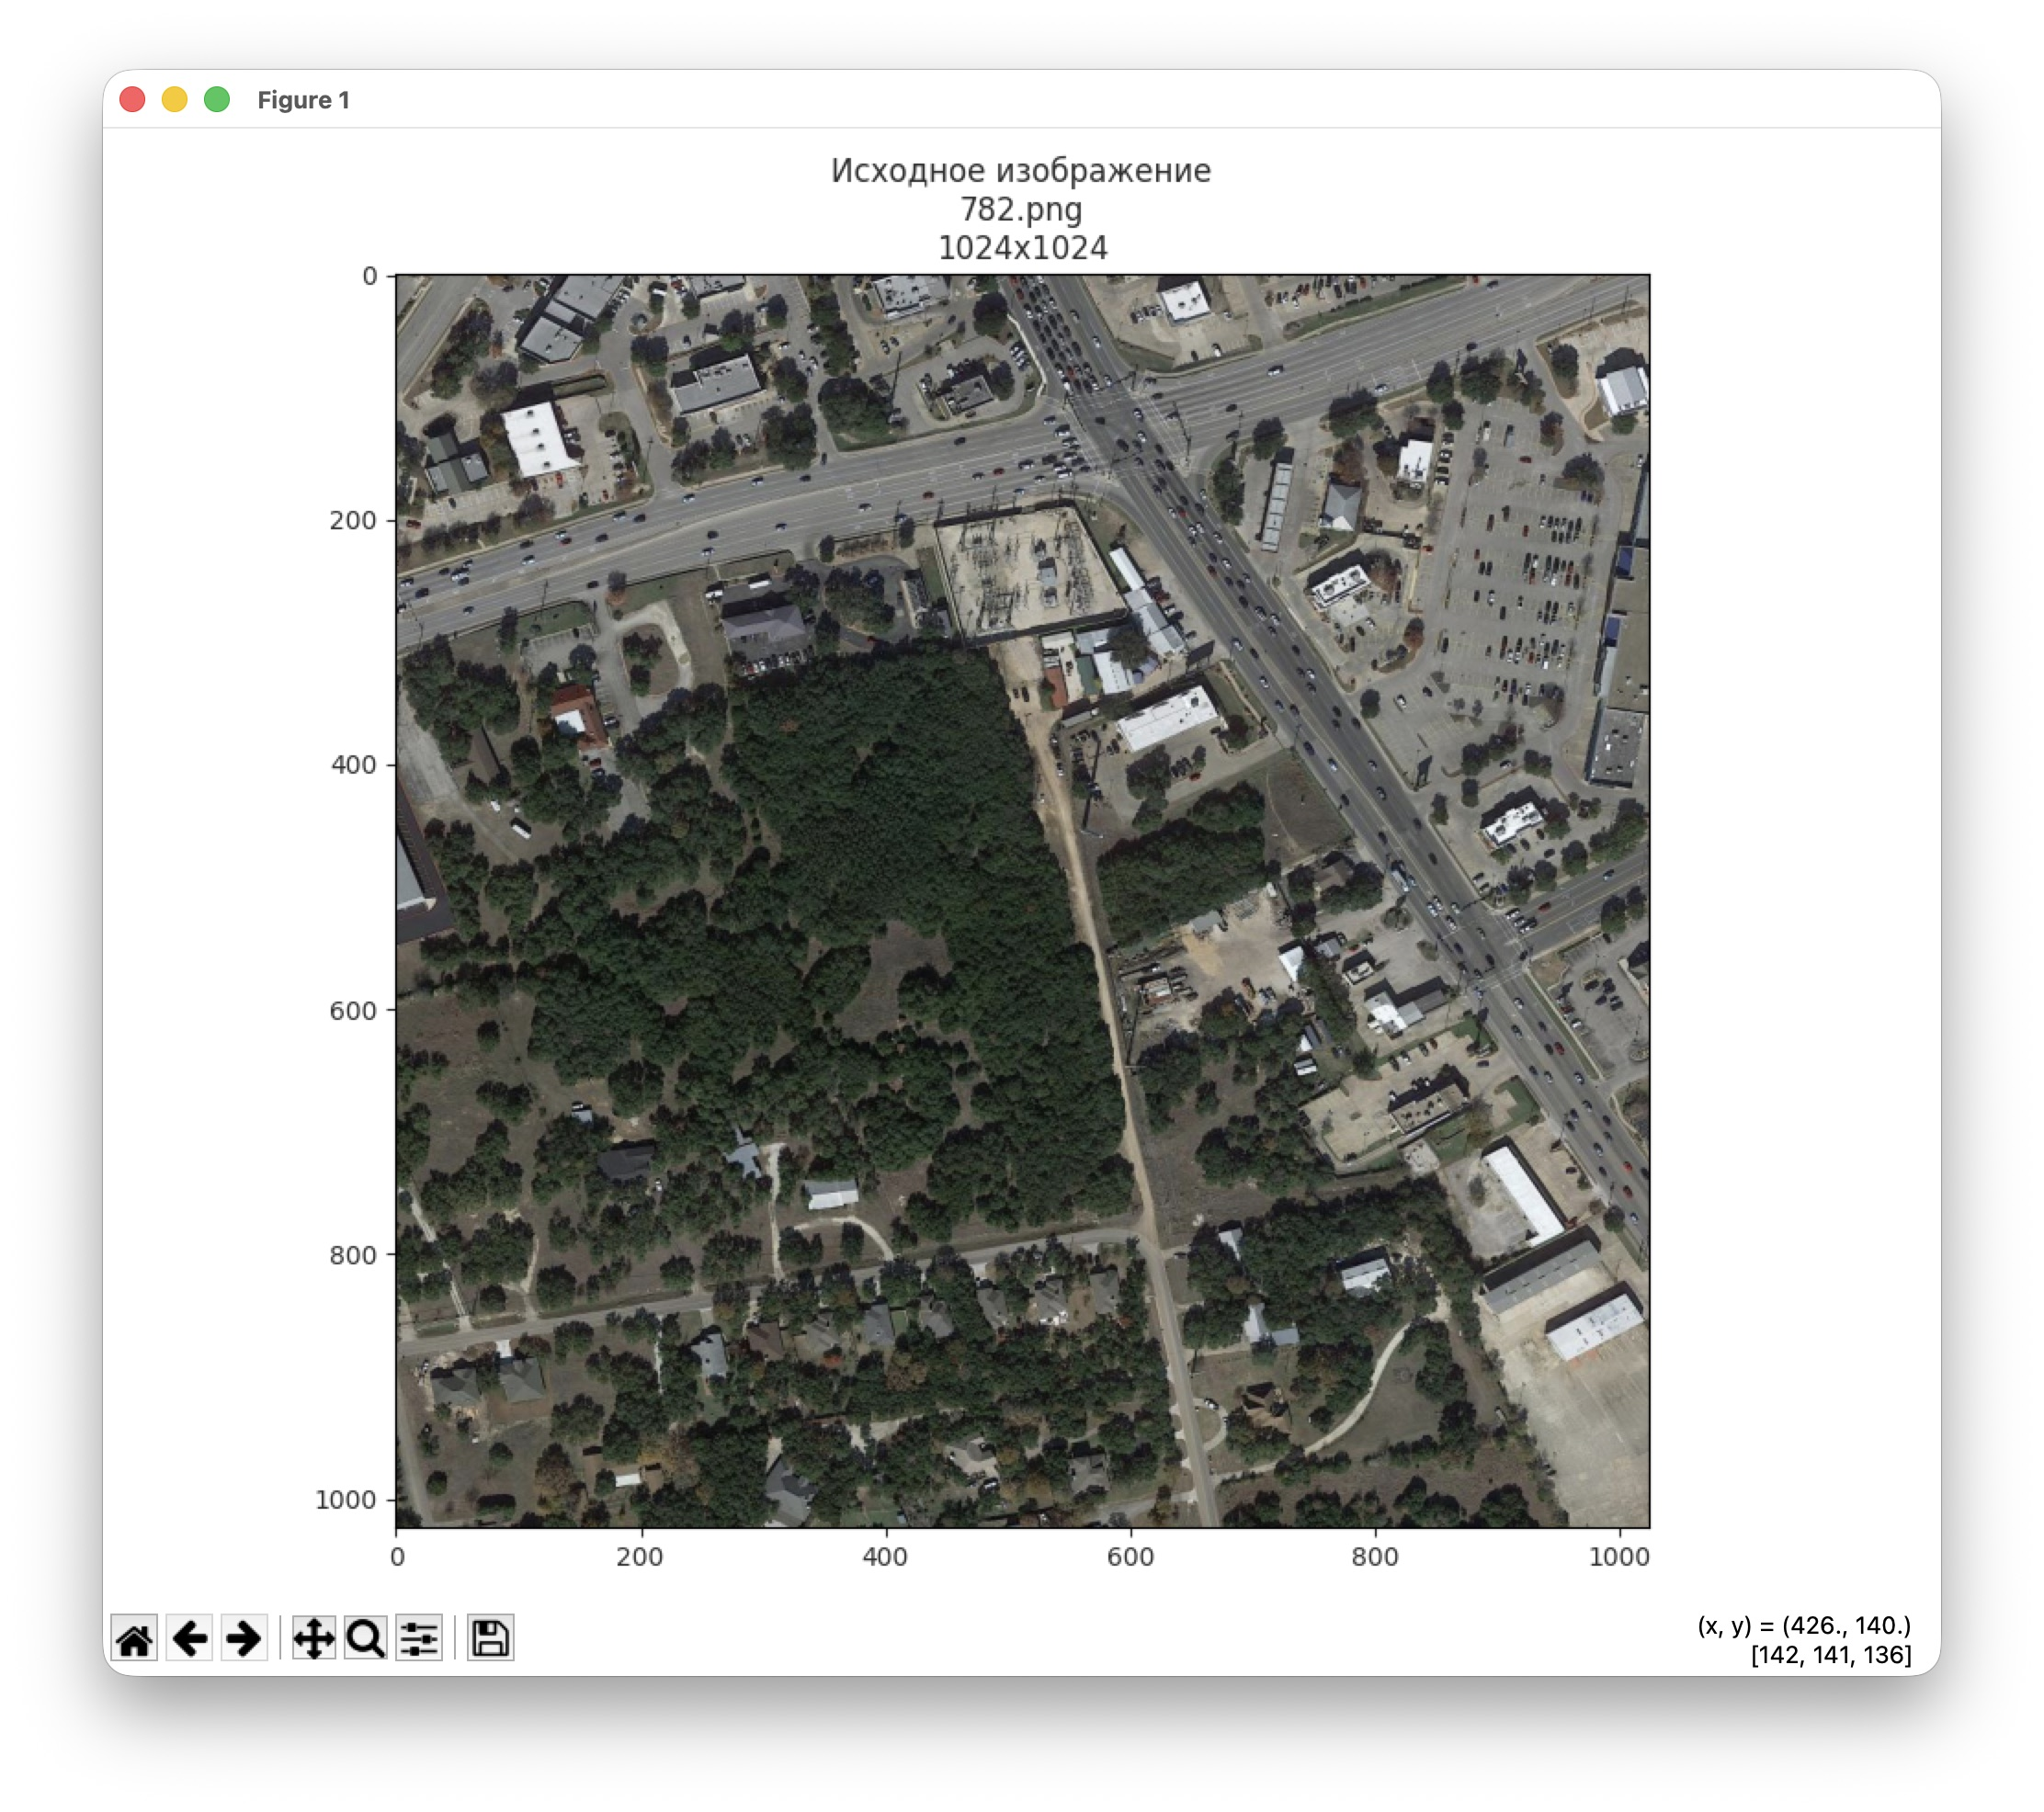
\includegraphics[width=0.6\linewidth]{images/technological/test_s5_in.jpeg}
    \caption{Входное изображение с разрешением $1024 \times 1024$}
    \label{fig:tech:test_s5_in}
\end{figure}

\begin{figure}[H]
    \centering
    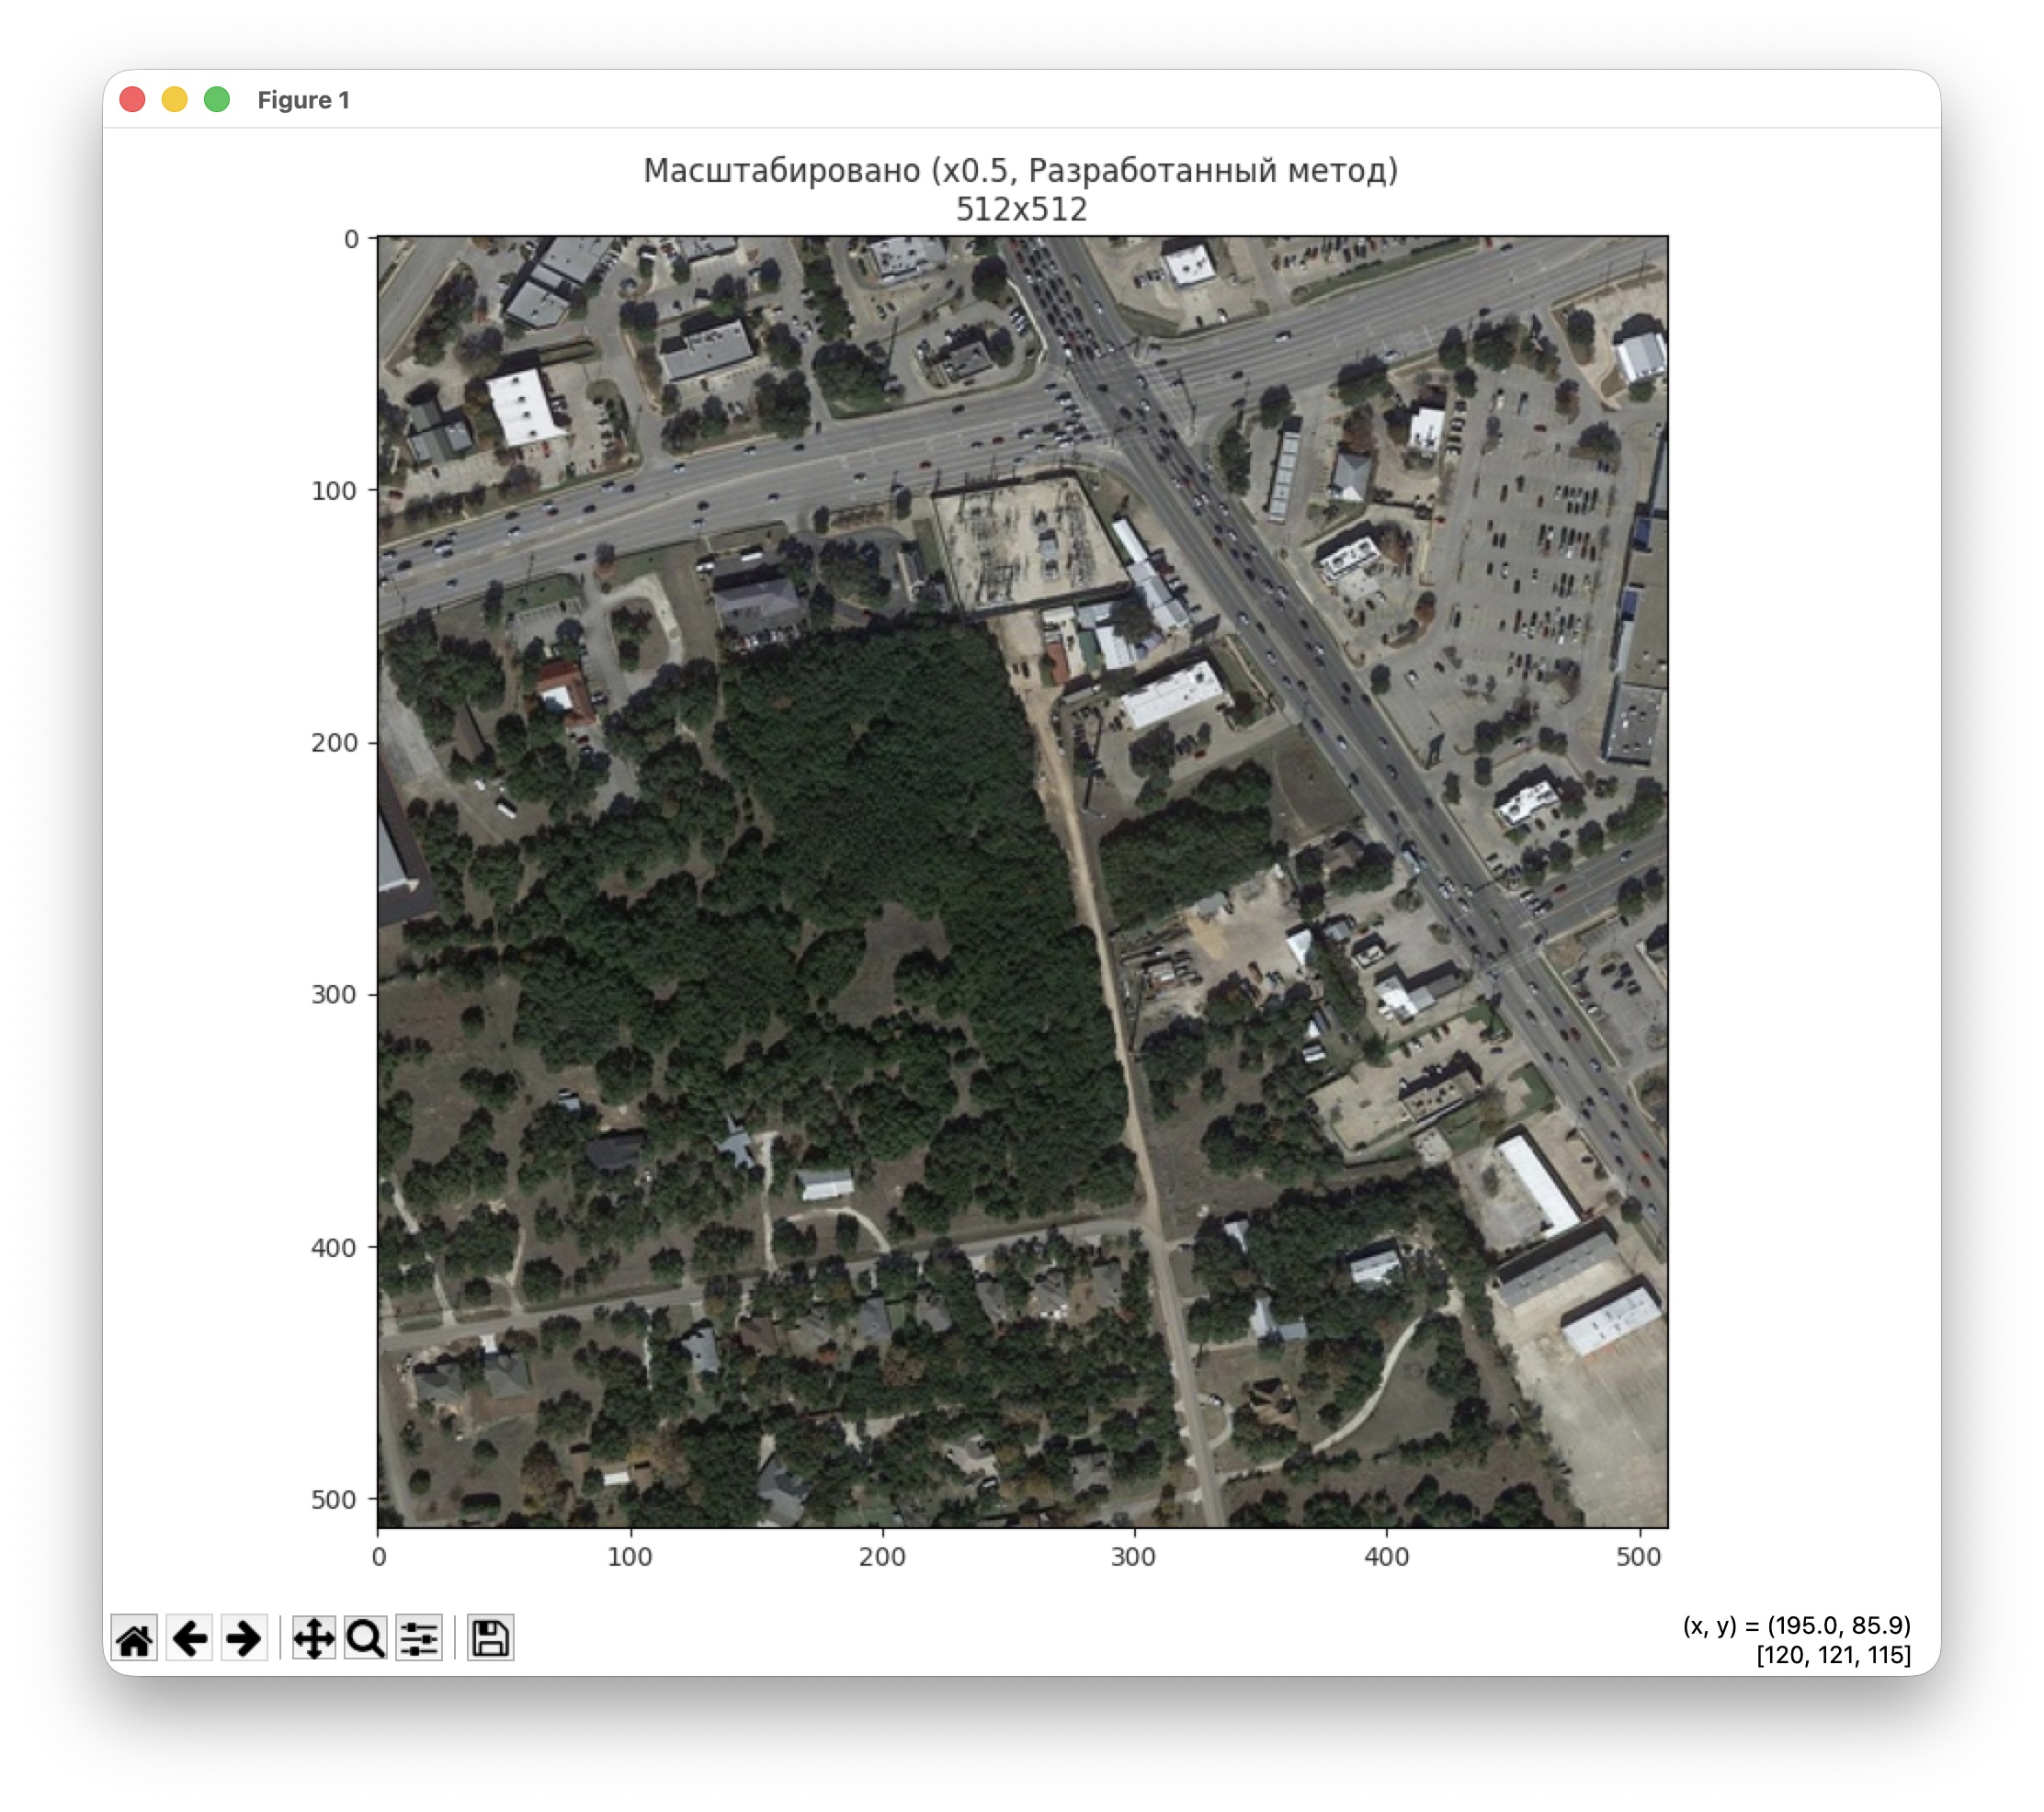
\includegraphics[width=0.6\linewidth]{images/technological/test_s5_out.jpeg}
    \caption{Изображение с разрешением $512 \times 512$ полученное масштабированием в 0.5 раз}
    \label{fig:tech:test_s5_out}
\end{figure}

Примеры работы масштабирования аэрофотоснимков показывают работоспособность повышения разрешения. Все нейронные сети работают с минимальным количеством артефактом, четко выделяя объекты. Также примеры показывают корректное повышение разрешения на произвольный коэффициент масштабирования с возможностью понижения разрешения. 

\section*{Вывод}
\addcontentsline{toc}{section}{Вывод}

В данном разделе был обоснован выбор средств реализации, описаны обучающая выборка и структура программного обеспечения. Также были приведены реализации разработанных алгоритмов и результаты тестирования программного обеспечения. 